\begin{table}
    \label{table:oval}
    \centering
    \begin{tabularx}{0.9\textwidth}{@{}XXXXXX@{}}
      \toprule
      \begin{tabular}{@{}c@{}}Ground Truth \\ 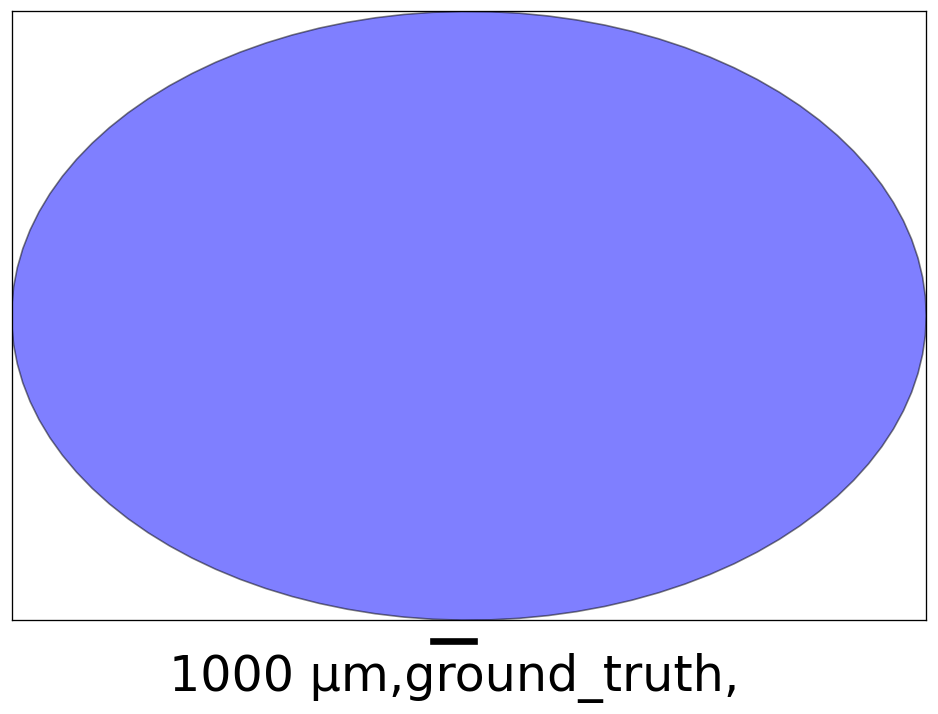
\includegraphics[width=0.13\textwidth]{examples_png/Oval.png}\end{tabular} & GPT-4o & Claude-3.5 & Llama-3-70B & Llama-3-405B & o1-preview \\
      \midrule
      SOLOMON & \includegraphics[width=0.13\textwidth]{./pool_all/png/gpt-4o_results/Oval.png} &  & \includegraphics[width=0.13\textwidth]{./pool_all/png/claude-3-5-sonnet-20240620_results/Oval.png} & 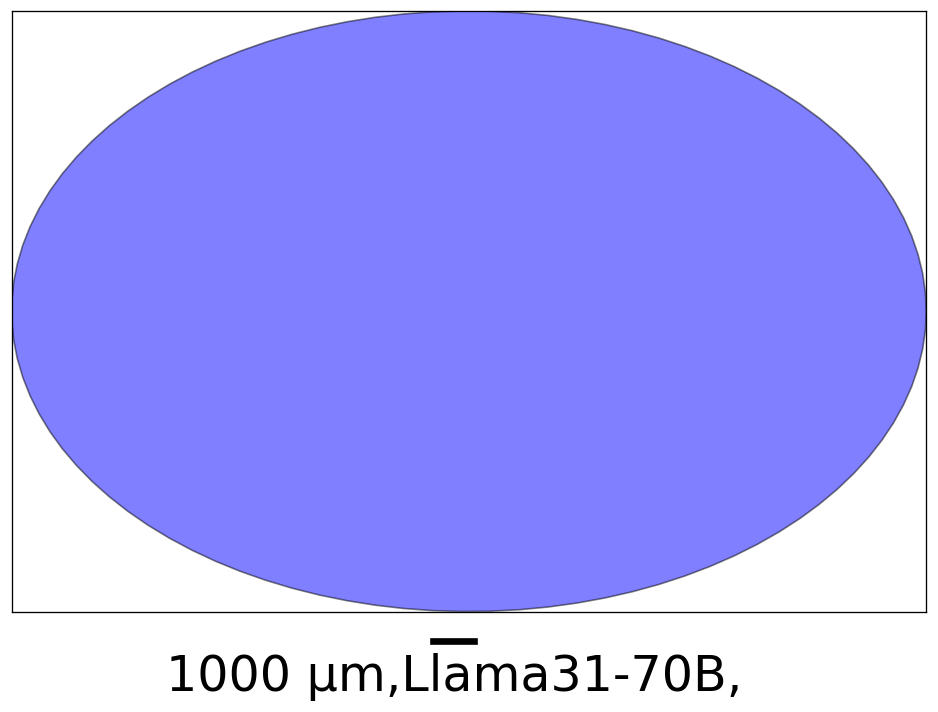
\includegraphics[width=0.13\textwidth]{./pool_all/png/watsonx_meta-llama_llama-3-1-70b-instruct_results/Oval.png} & 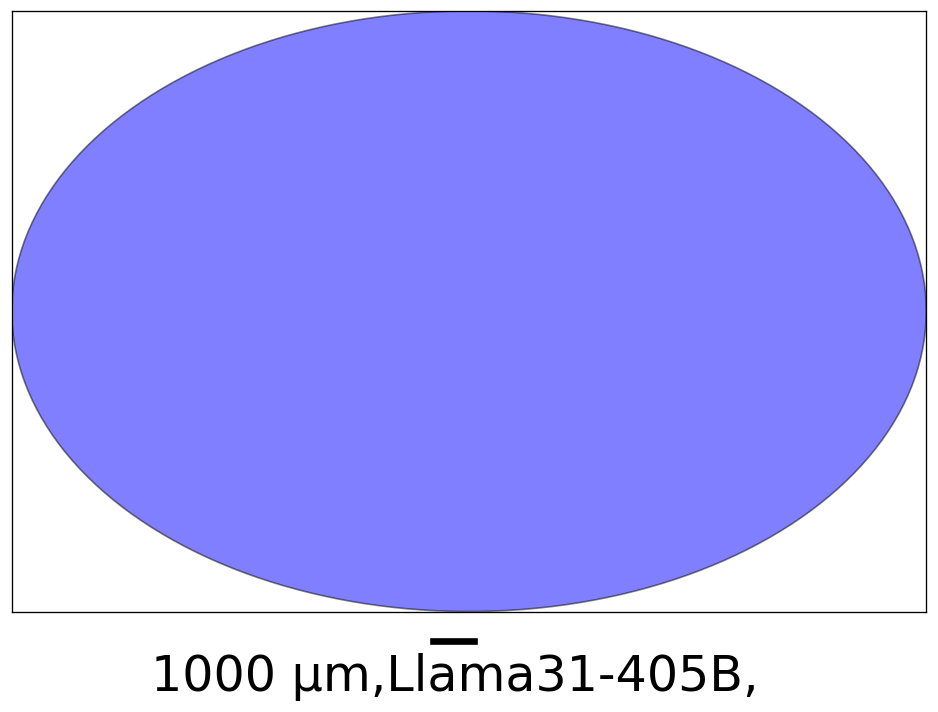
\includegraphics[width=0.13\textwidth]{./pool_all/png/watsonx_meta-llama_llama-3-405b-instruct_results/Oval.png} \\
      \begin{tabular}{@{}c@{}}Single LLM \\ Baseline \\ Run 1\end{tabular} & 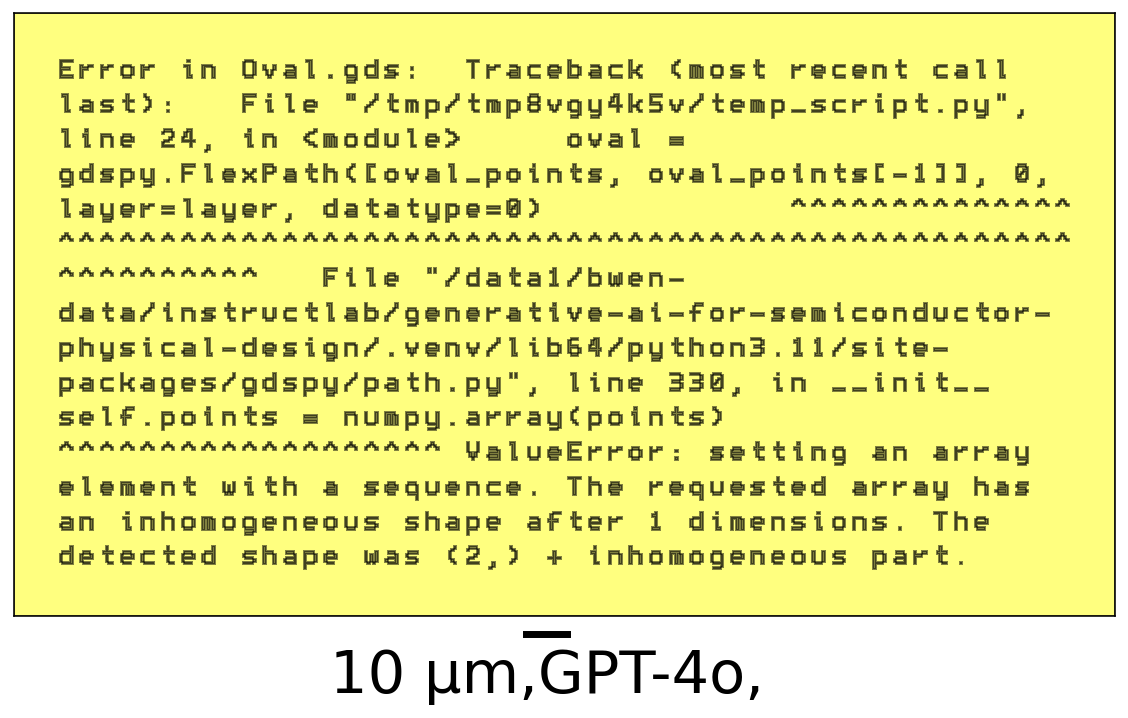
\includegraphics[width=0.13\textwidth]{./run_1/png/gpt-4o_results/Oval.png} & 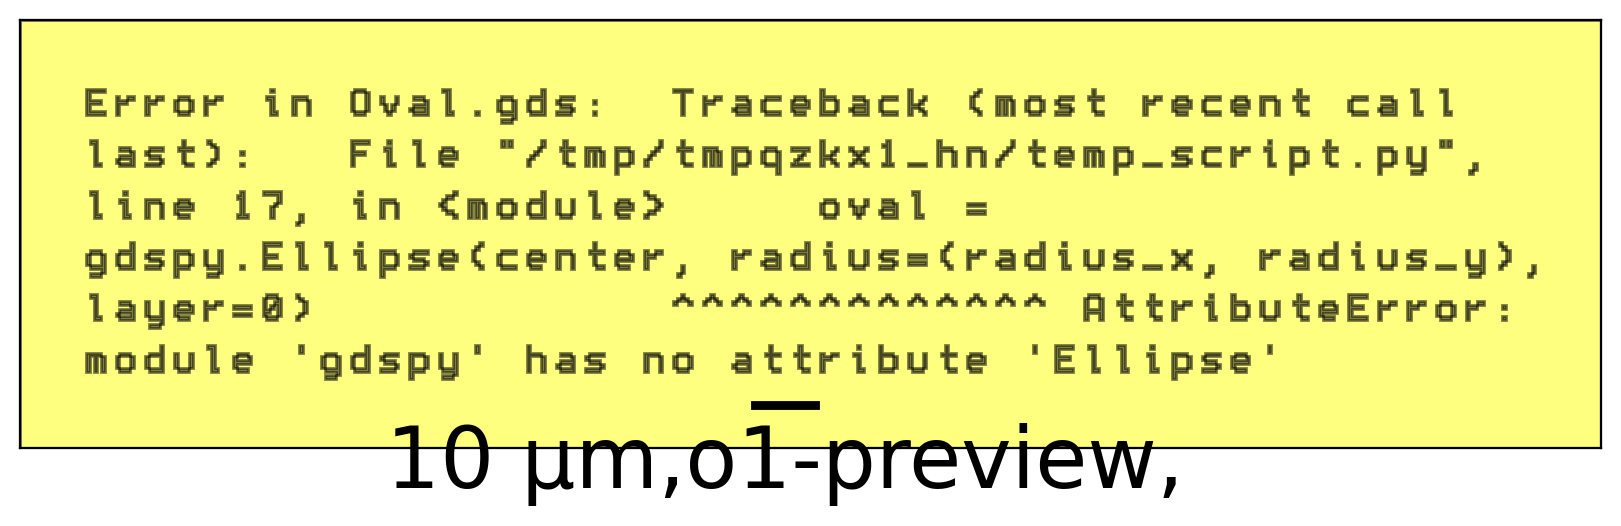
\includegraphics[width=0.13\textwidth]{./run_1/png/o1-preview_results/Oval.png} & 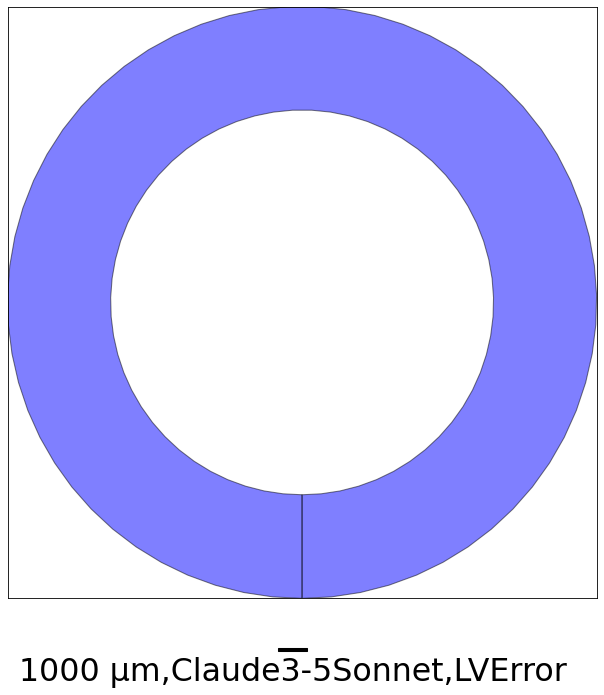
\includegraphics[width=0.13\textwidth]{./run_1/png/claude-3-5-sonnet-20240620_results/Oval.png} & 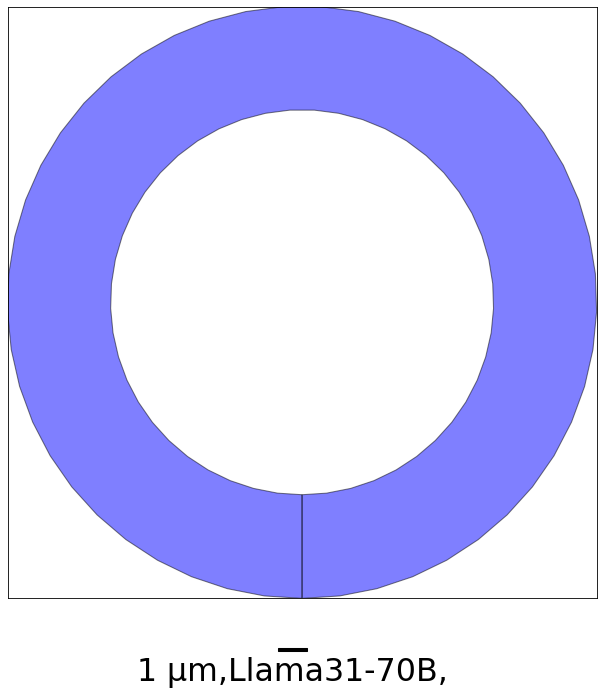
\includegraphics[width=0.13\textwidth]{./run_1/png/watsonx_meta-llama_llama-3-1-70b-instruct_results/Oval.png} & 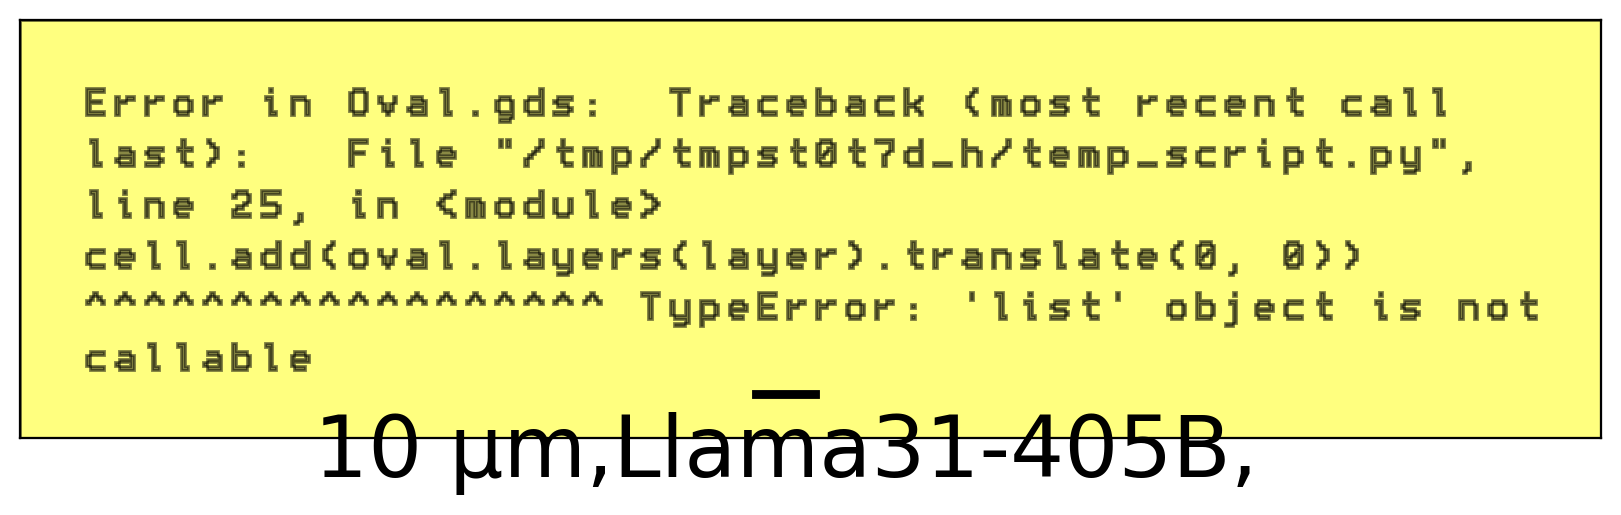
\includegraphics[width=0.13\textwidth]{./run_1/png/watsonx_meta-llama_llama-3-405b-instruct_results/Oval.png} \\
      \begin{tabular}{@{}c@{}}Single LLM \\ Baseline \\ Run 2\end{tabular} & 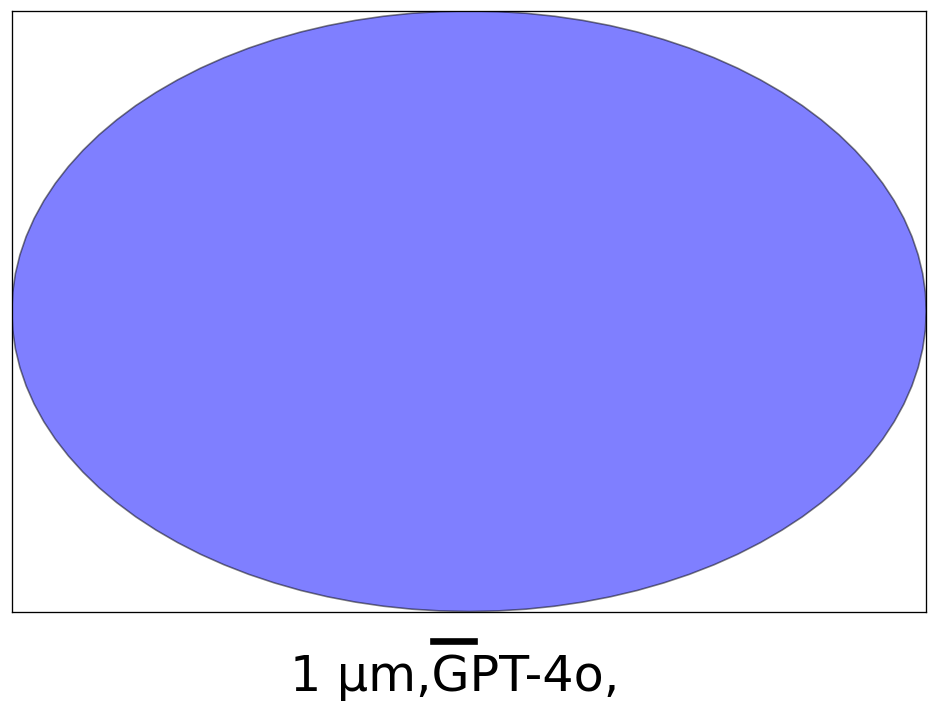
\includegraphics[width=0.13\textwidth]{./run_2/png/gpt-4o_results/Oval.png} & 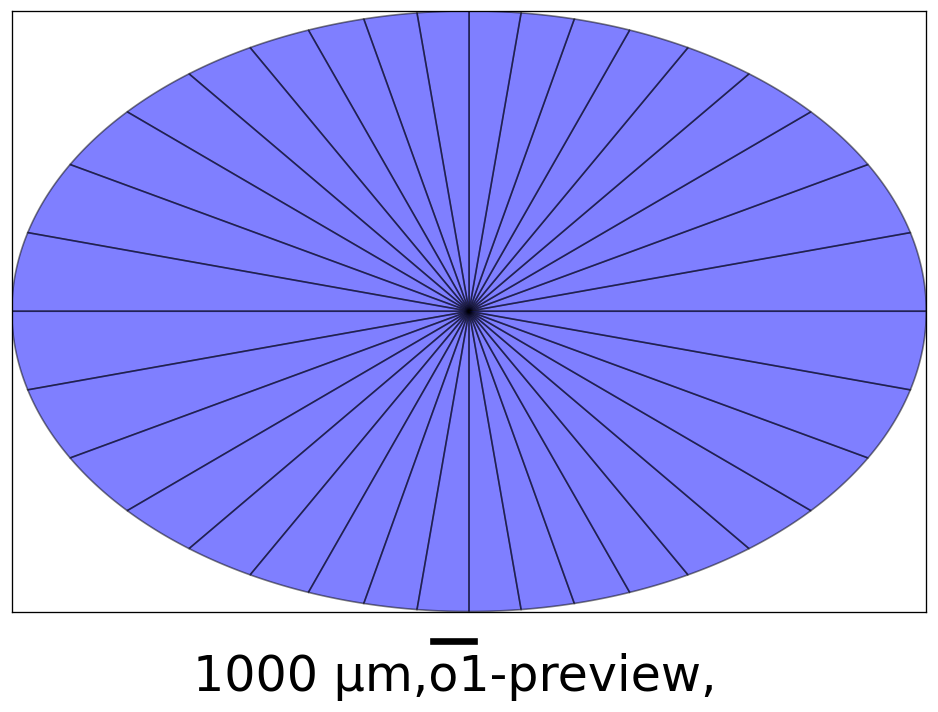
\includegraphics[width=0.13\textwidth]{./run_2/png/o1-preview_results/Oval.png} & 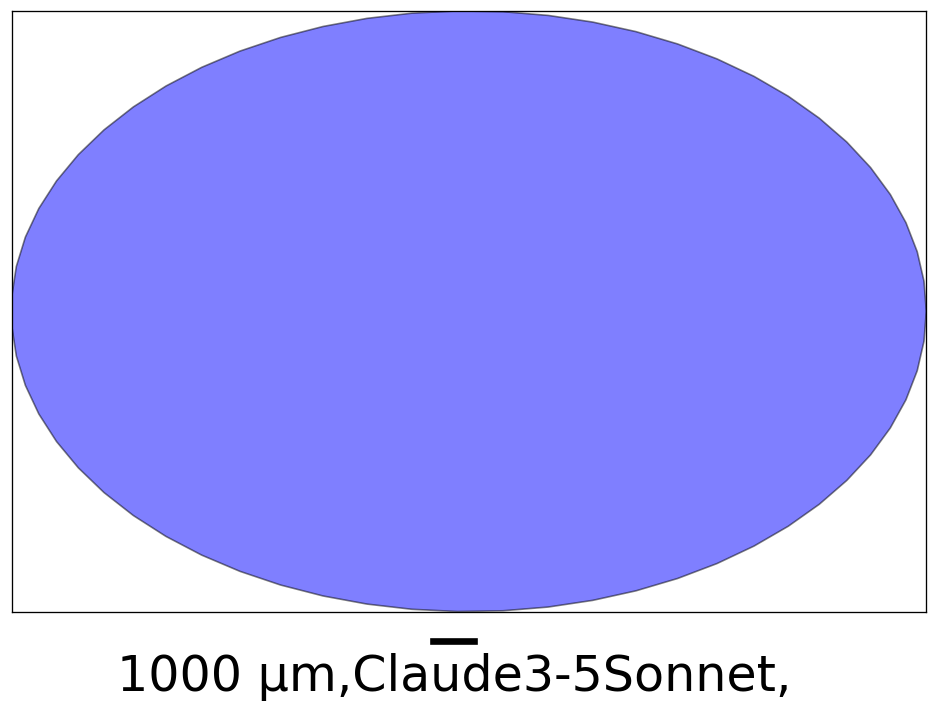
\includegraphics[width=0.13\textwidth]{./run_2/png/claude-3-5-sonnet-20240620_results/Oval.png} & 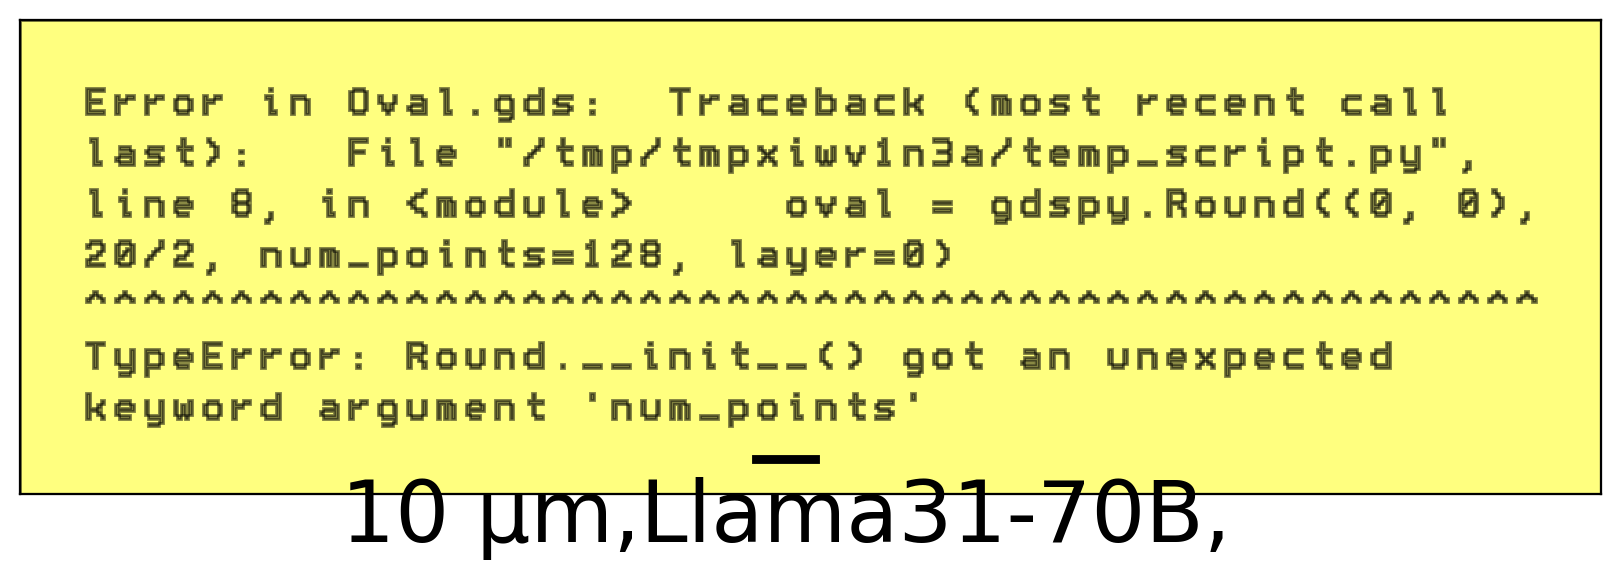
\includegraphics[width=0.13\textwidth]{./run_2/png/watsonx_meta-llama_llama-3-1-70b-instruct_results/Oval.png} & 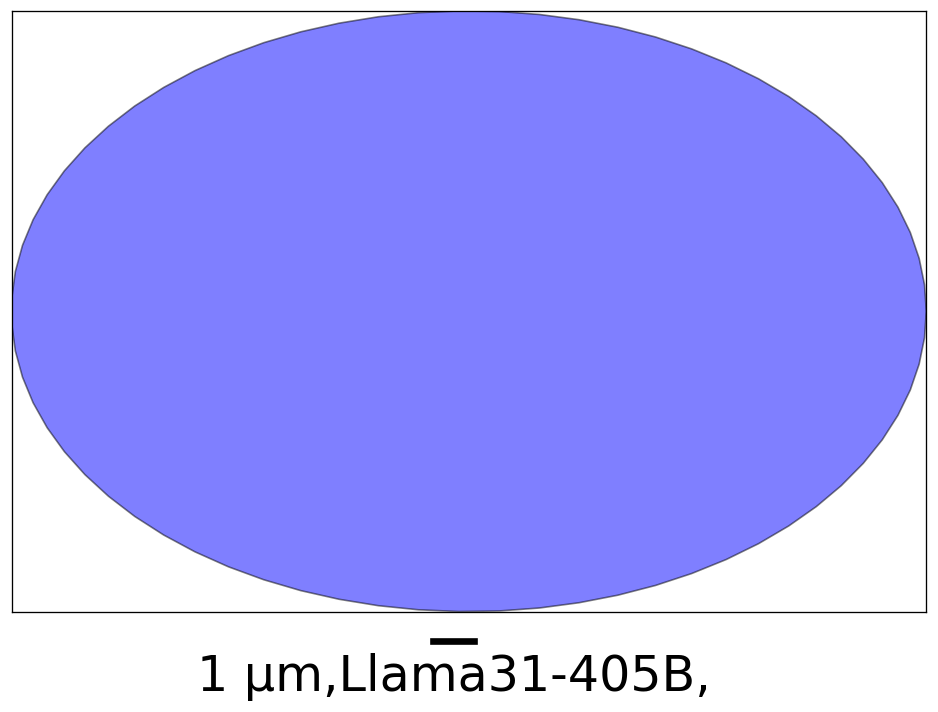
\includegraphics[width=0.13\textwidth]{./run_2/png/watsonx_meta-llama_llama-3-405b-instruct_results/Oval.png} \\
      \begin{tabular}{@{}c@{}}Single LLM \\ Baseline \\ Run 3\end{tabular} & 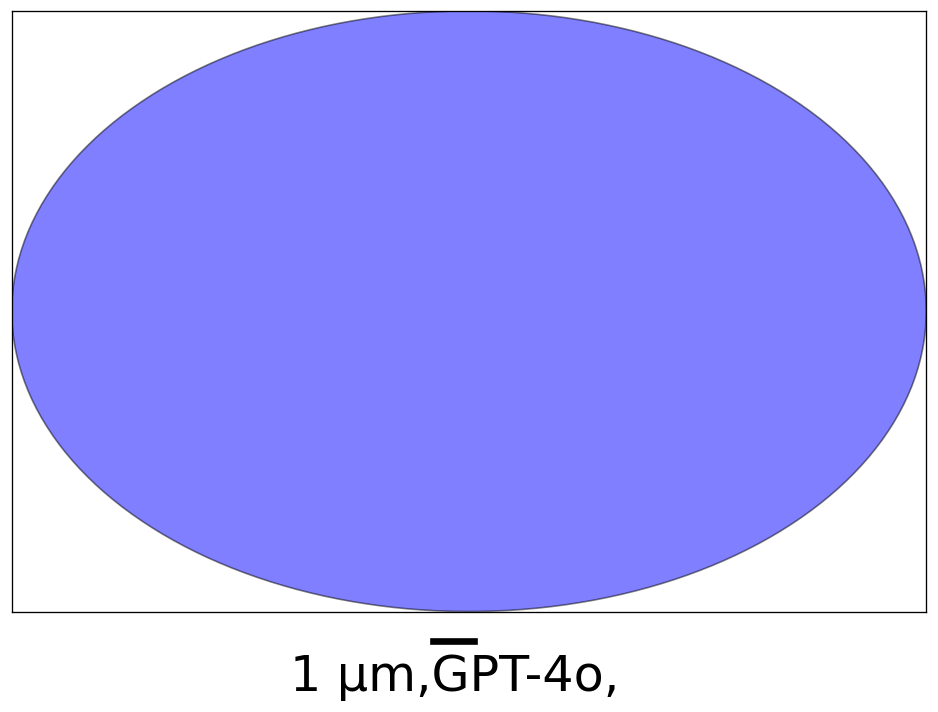
\includegraphics[width=0.13\textwidth]{./run_3/png/gpt-4o_results/Oval.png} & 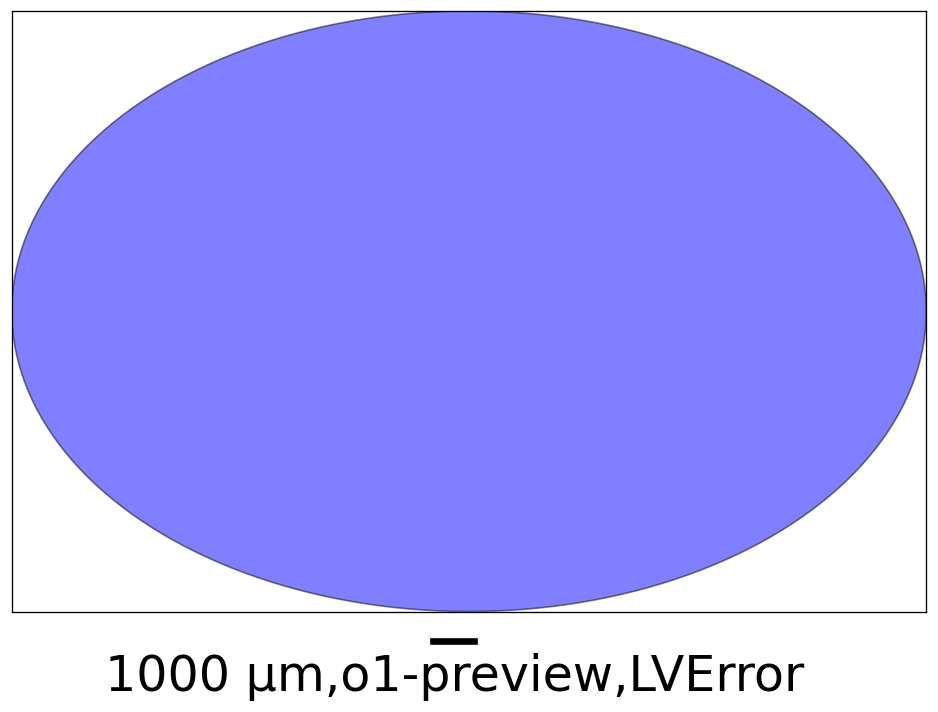
\includegraphics[width=0.13\textwidth]{./run_3/png/o1-preview_results/Oval.png} & \includegraphics[width=0.13\textwidth]{./run_3/png/claude-3-5-sonnet-20240620_results/Oval.png} & 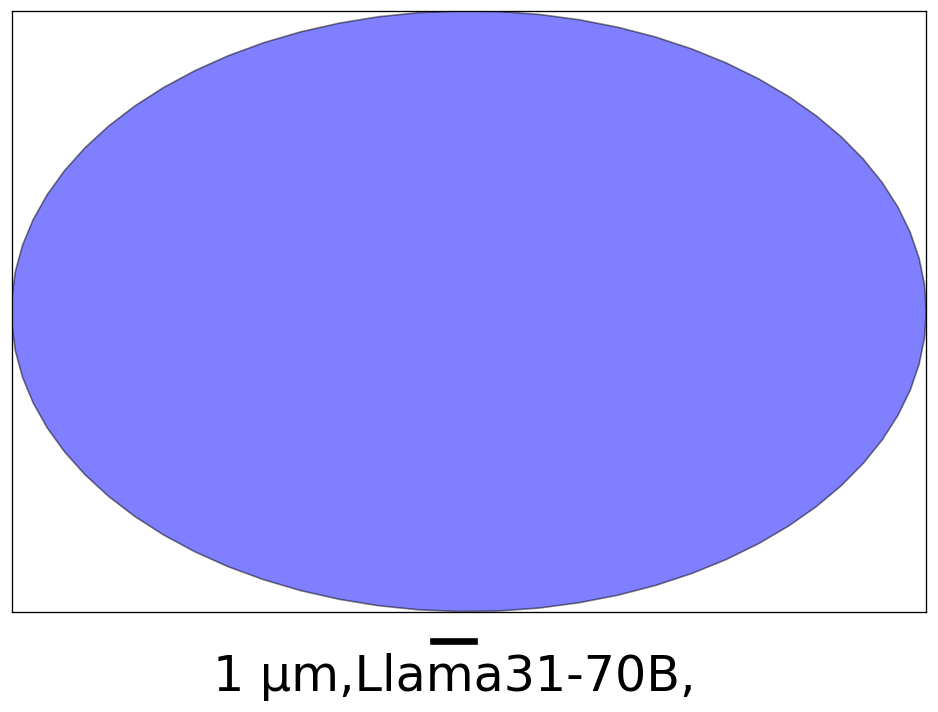
\includegraphics[width=0.13\textwidth]{./run_3/png/watsonx_meta-llama_llama-3-1-70b-instruct_results/Oval.png} & 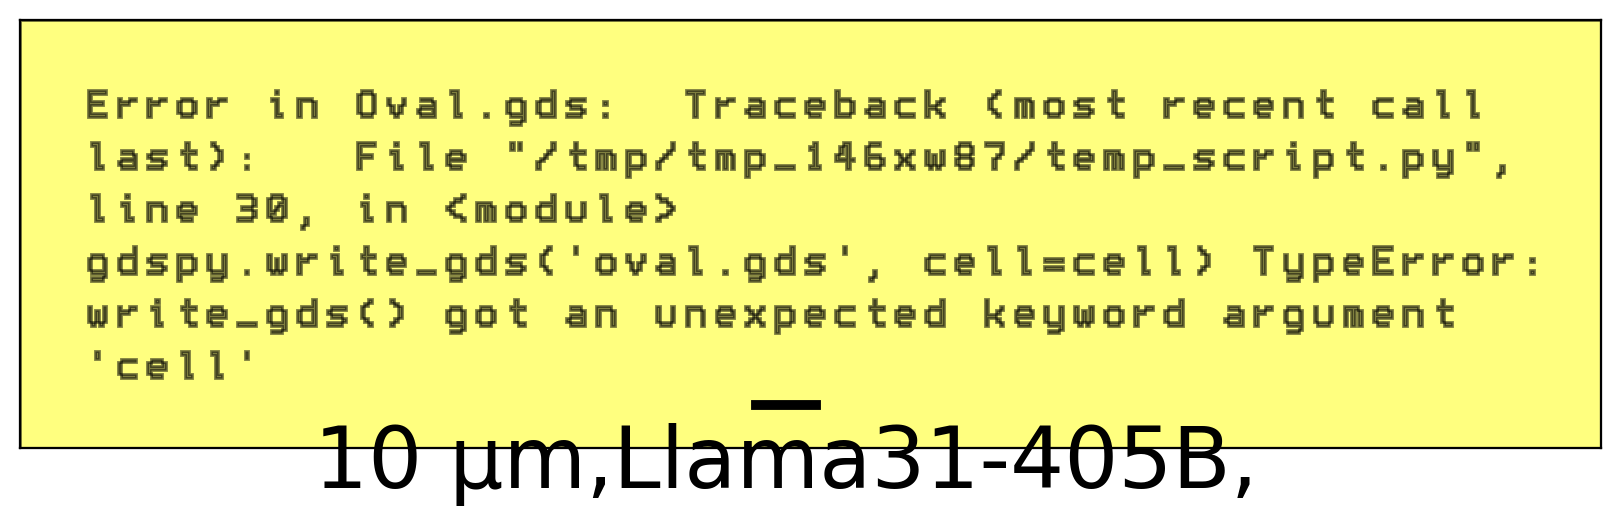
\includegraphics[width=0.13\textwidth]{./run_3/png/watsonx_meta-llama_llama-3-405b-instruct_results/Oval.png} \\
      \begin{tabular}{@{}c@{}}Single LLM \\ Baseline \\ Run 4\end{tabular} & \includegraphics[width=0.13\textwidth]{./run_4/png/gpt-4o_results/Oval.png} & 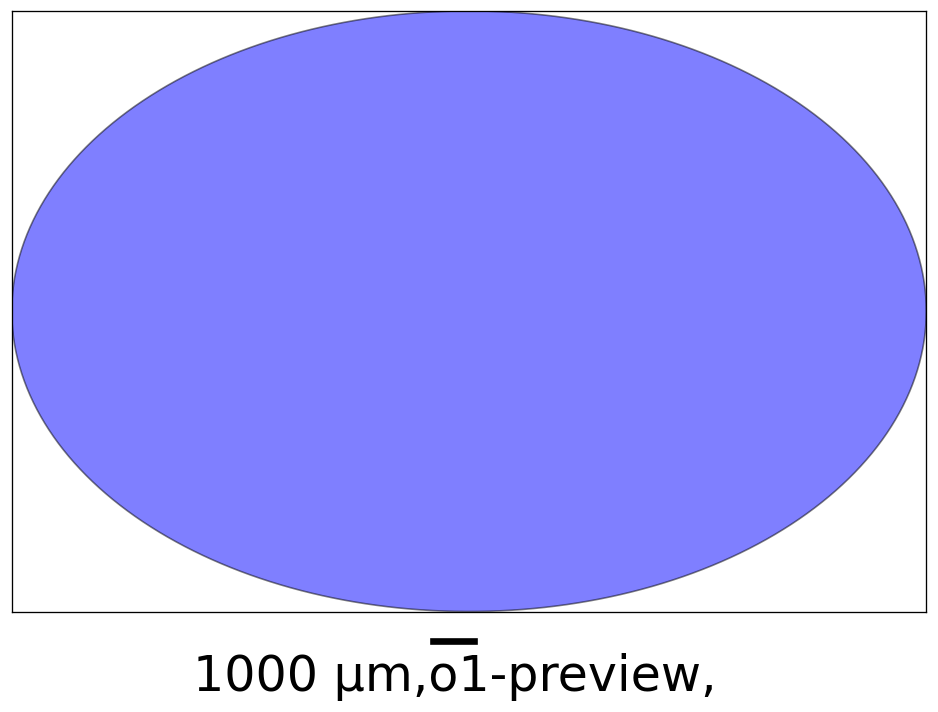
\includegraphics[width=0.13\textwidth]{./run_4/png/o1-preview_results/Oval.png} & 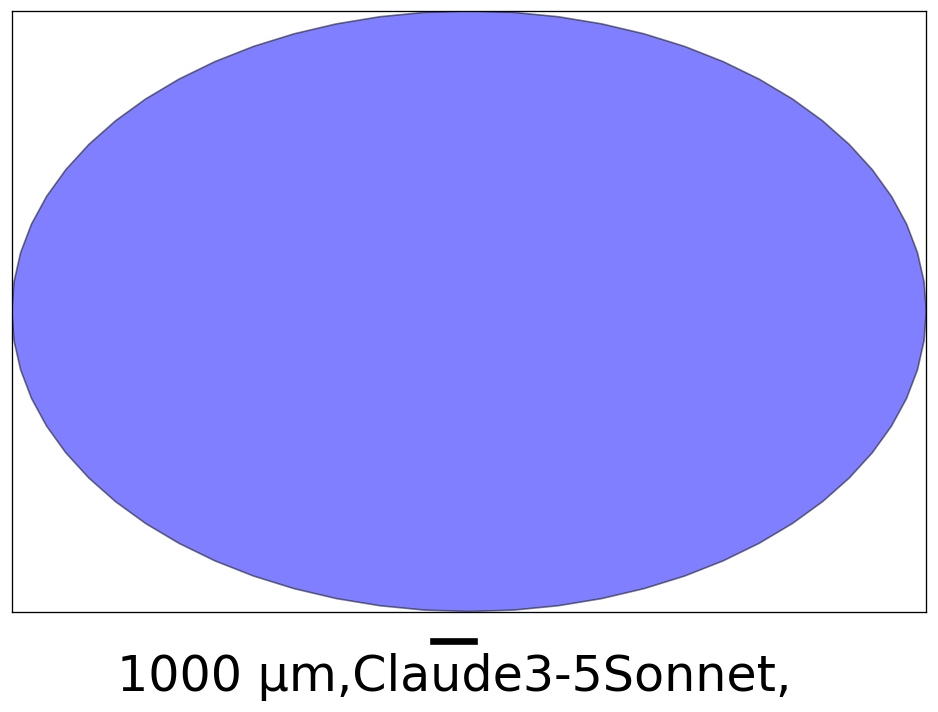
\includegraphics[width=0.13\textwidth]{./run_4/png/claude-3-5-sonnet-20240620_results/Oval.png} & 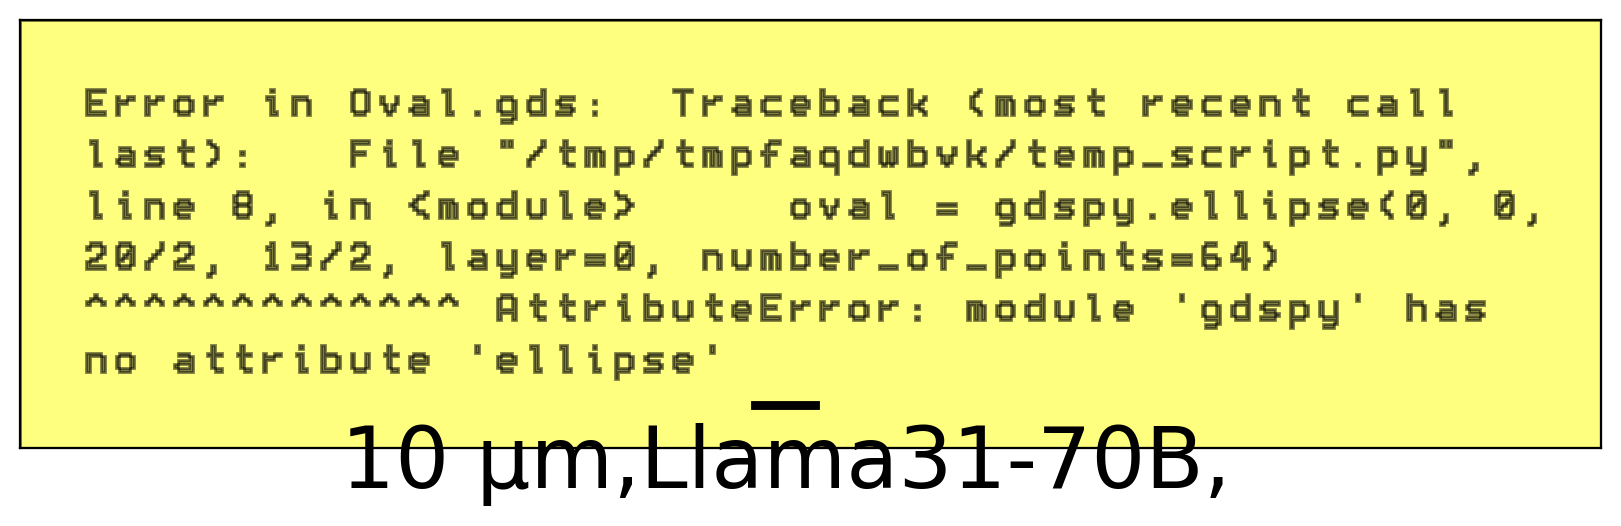
\includegraphics[width=0.13\textwidth]{./run_4/png/watsonx_meta-llama_llama-3-1-70b-instruct_results/Oval.png} & 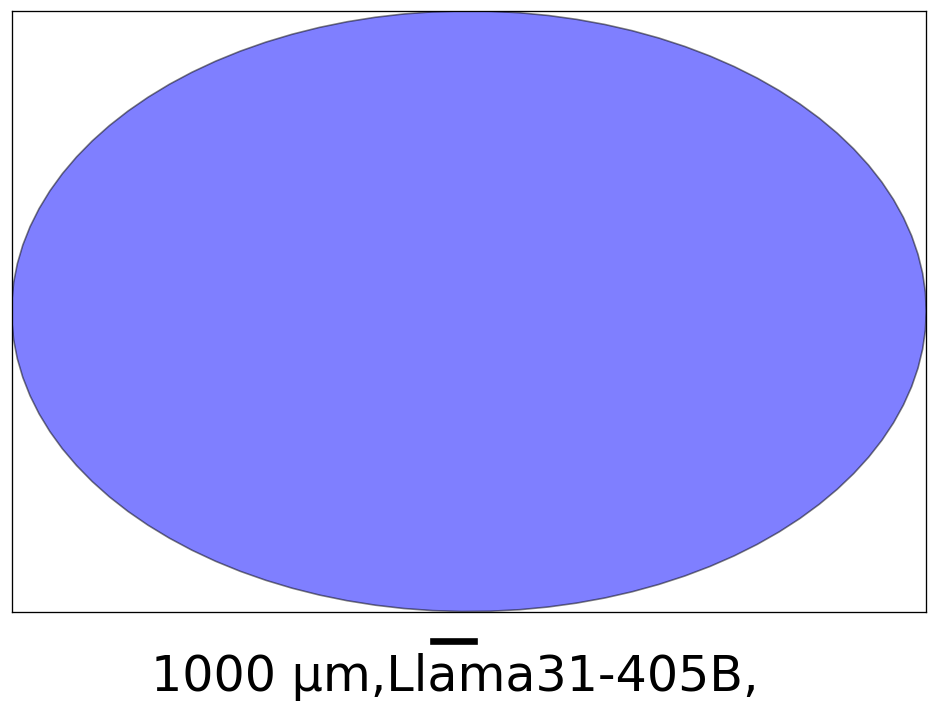
\includegraphics[width=0.13\textwidth]{./run_4/png/watsonx_meta-llama_llama-3-405b-instruct_results/Oval.png} \\
      \begin{tabular}{@{}c@{}}Single LLM \\ Baseline \\ Run 5\end{tabular} & 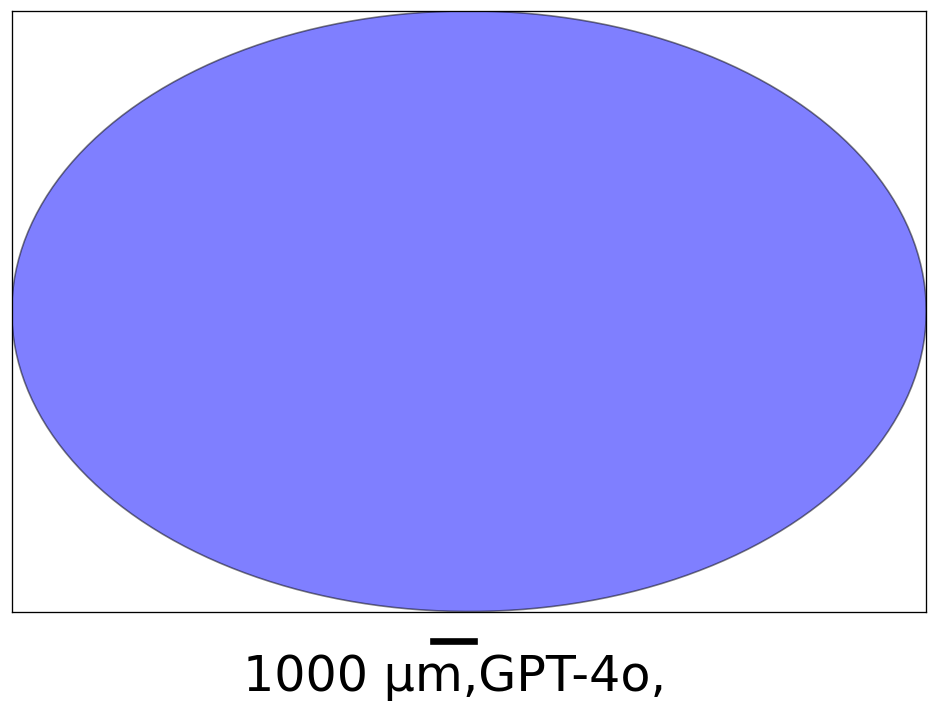
\includegraphics[width=0.13\textwidth]{./run_5/png/gpt-4o_results/Oval.png} & 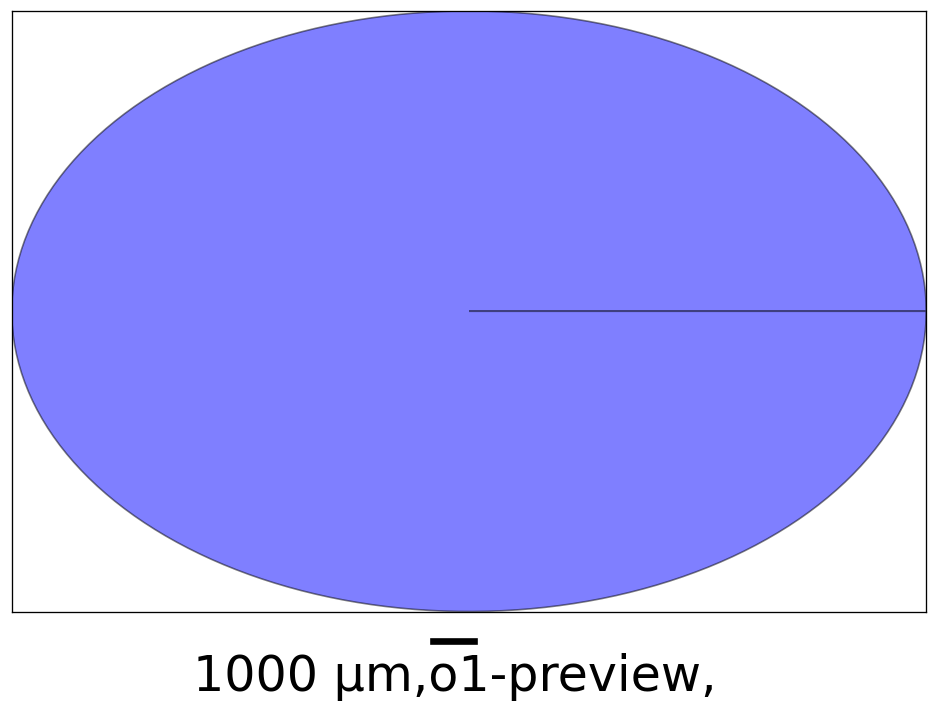
\includegraphics[width=0.13\textwidth]{./run_5/png/o1-preview_results/Oval.png} & 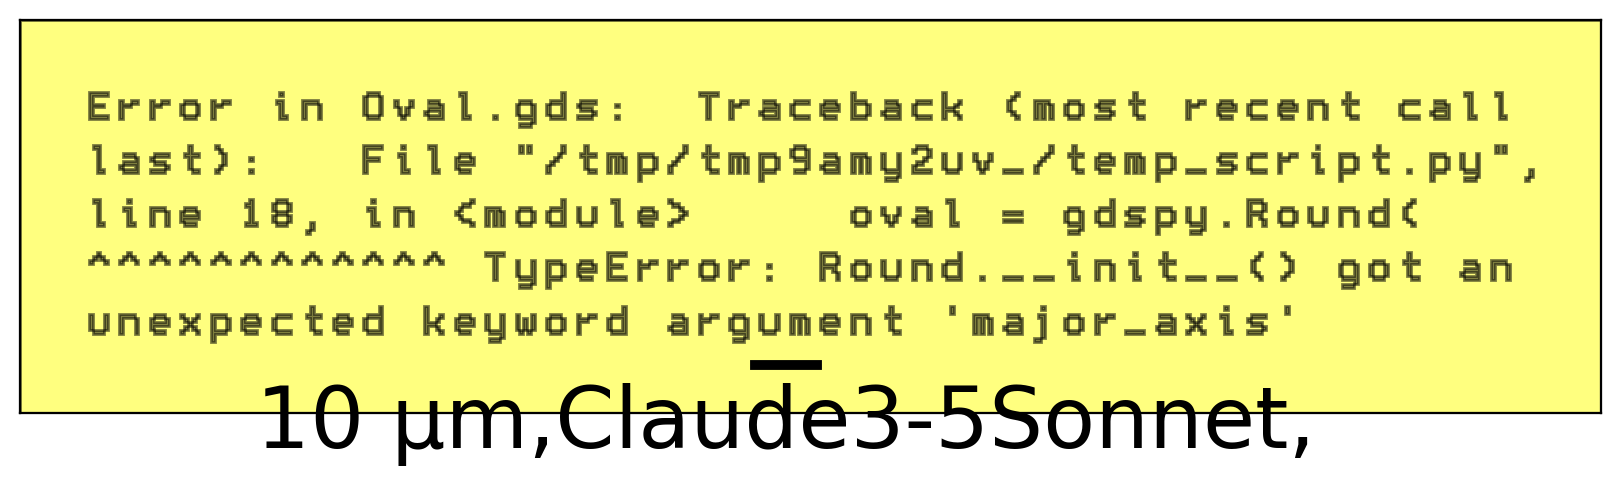
\includegraphics[width=0.13\textwidth]{./run_5/png/claude-3-5-sonnet-20240620_results/Oval.png} & 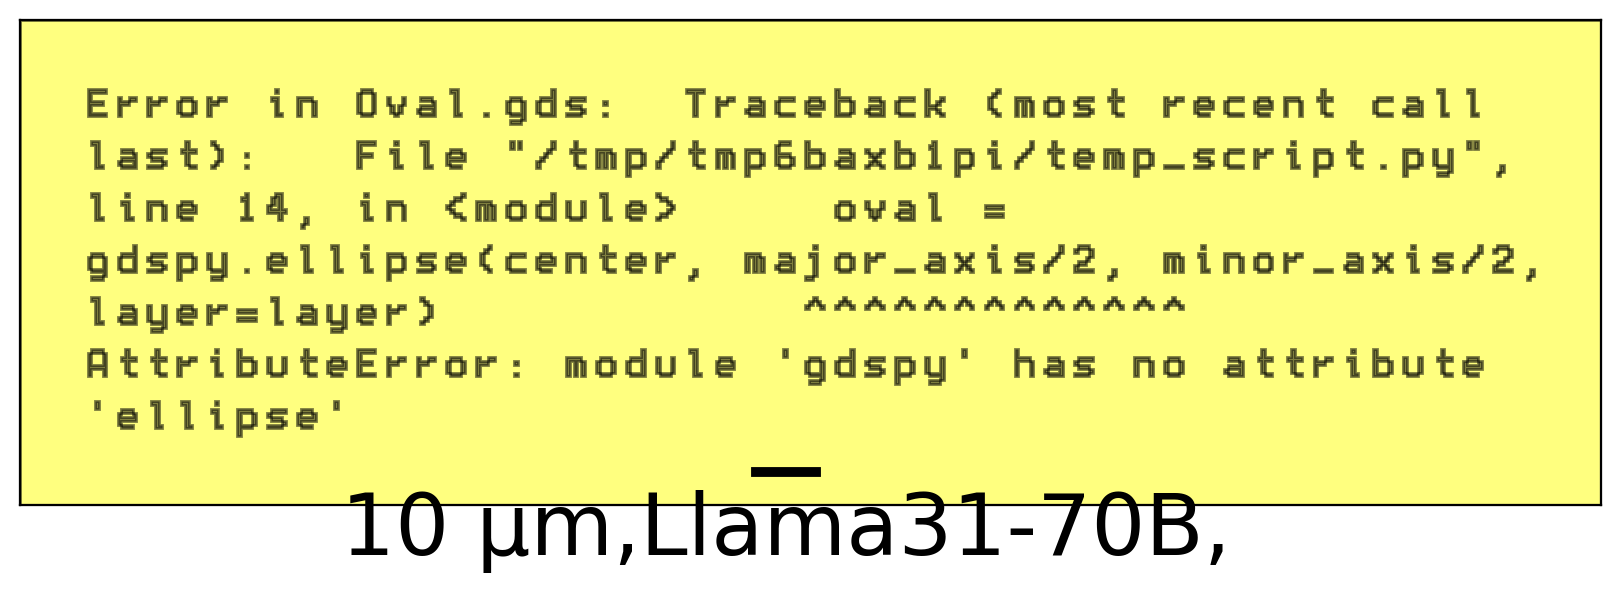
\includegraphics[width=0.13\textwidth]{./run_5/png/watsonx_meta-llama_llama-3-1-70b-instruct_results/Oval.png} & 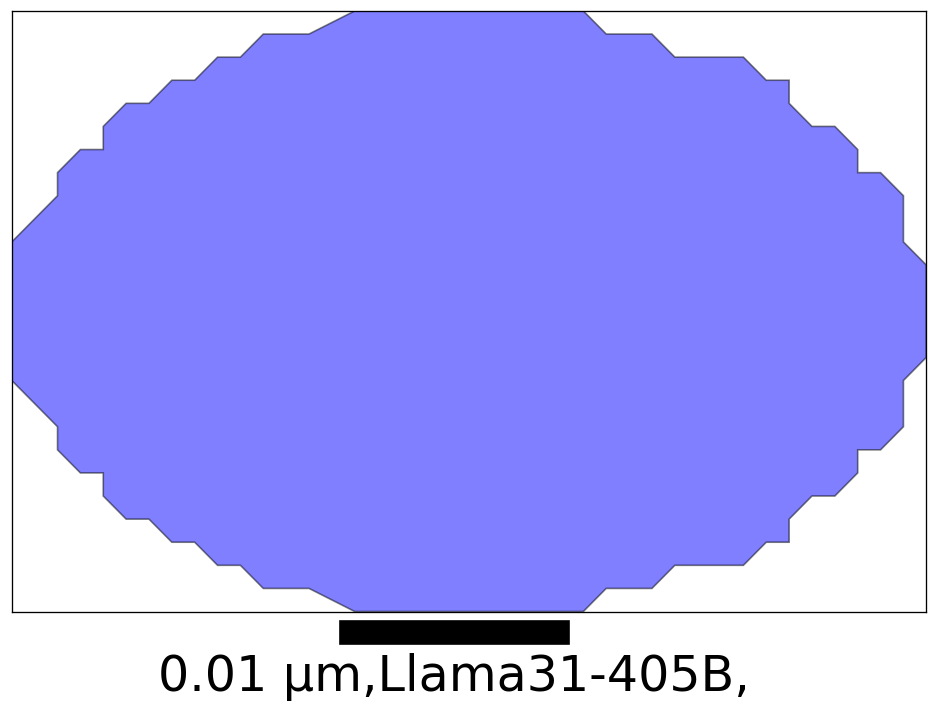
\includegraphics[width=0.13\textwidth]{./run_5/png/watsonx_meta-llama_llama-3-405b-instruct_results/Oval.png} \\
      \bottomrule
    \end{tabularx}
    \caption{Oval Task Question: Generate an oval with major axis of 20 mm, minor axis of 13 mm, on layer 0, center at 0,0.}
  \end{table}
  
  \begin{table}
    \label{table:arrow}
    \centering
    \begin{tabularx}{0.9\textwidth}{@{}XXXXXX@{}}
      \toprule
      \begin{tabular}{@{}c@{}}Ground Truth \\ 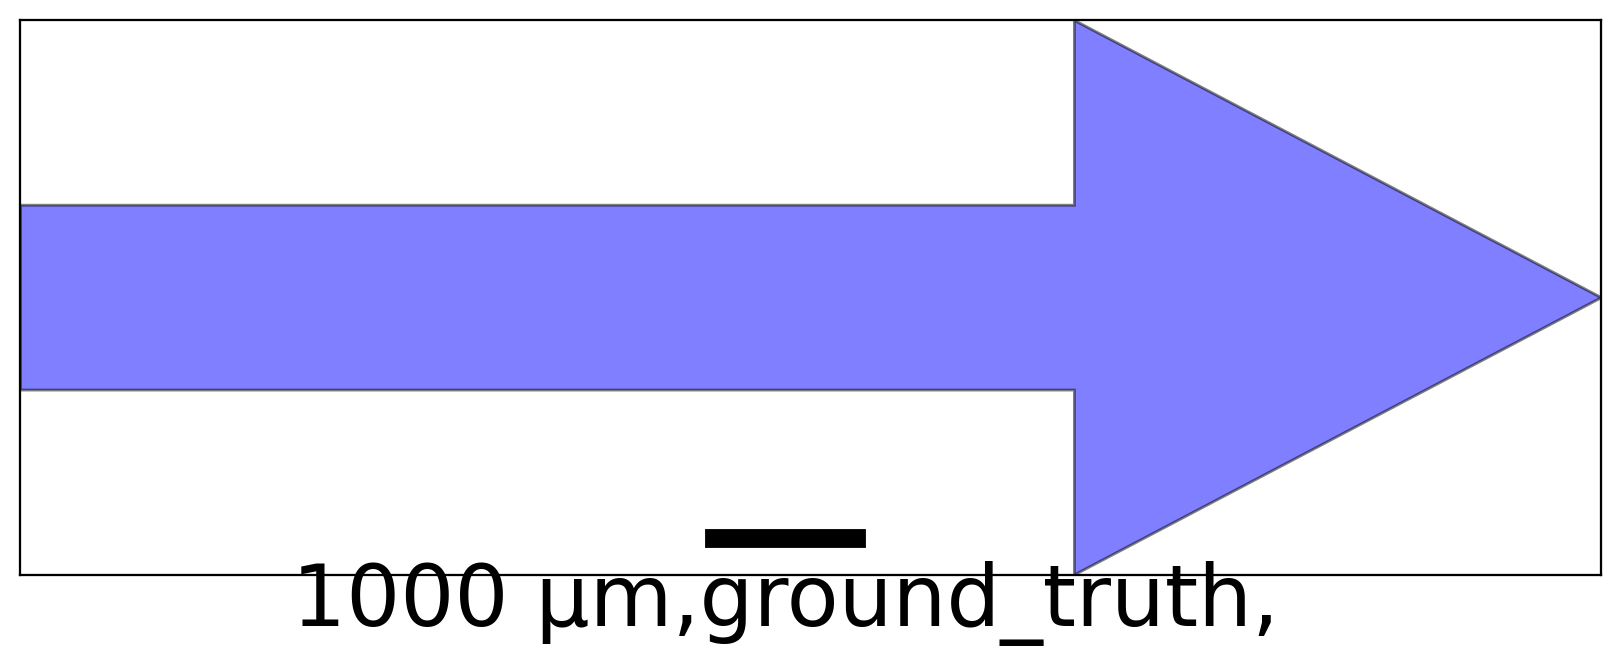
\includegraphics[width=0.13\textwidth]{examples_png/Arrow.png}\end{tabular} & GPT-4o & Claude-3.5 & Llama-3-70B & Llama-3-405B & o1-preview \\
      \midrule
      SOLOMON & 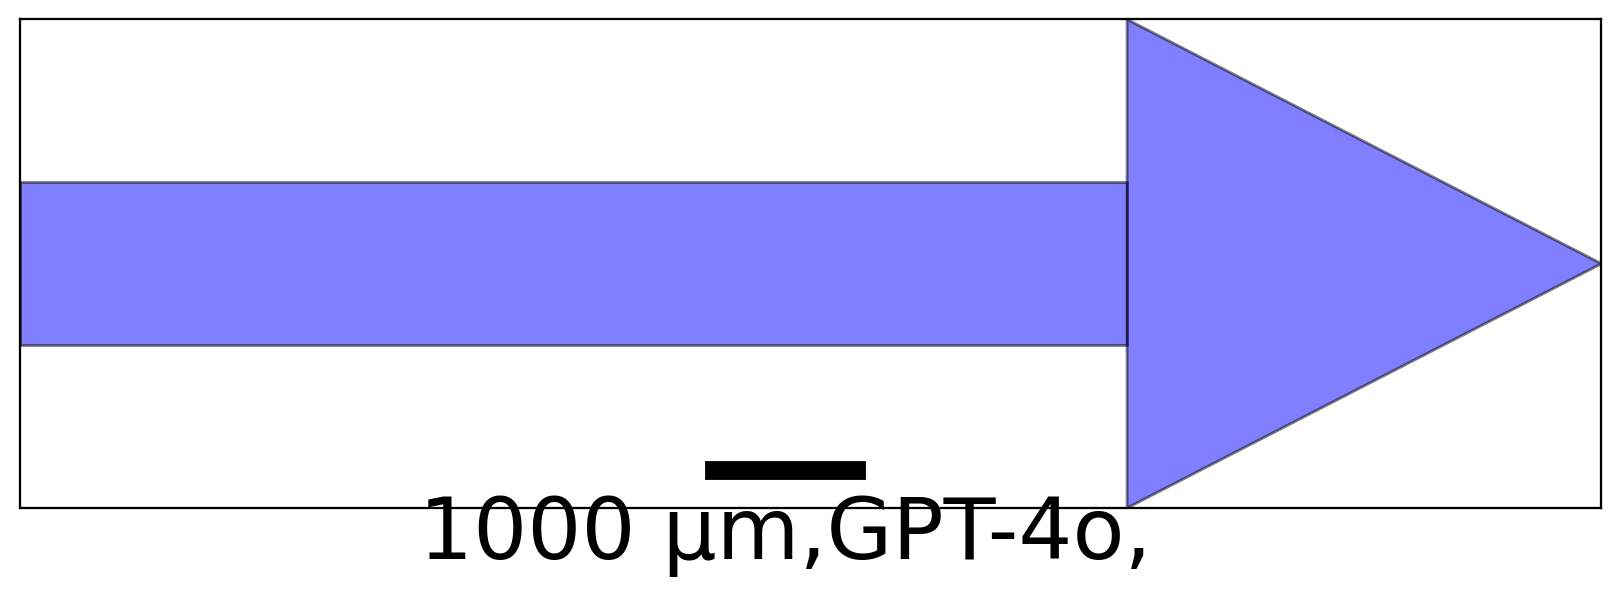
\includegraphics[width=0.13\textwidth]{./pool_all/png/gpt-4o_results/Arrow.png} &  & 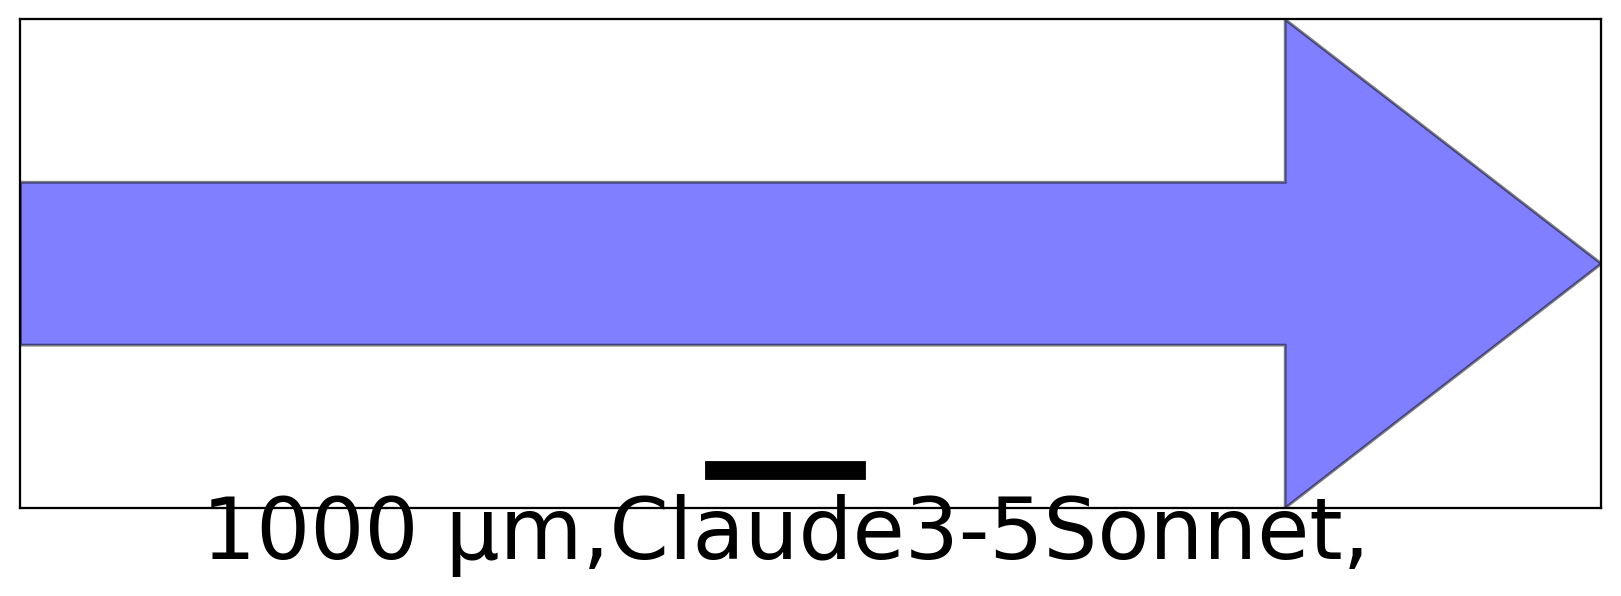
\includegraphics[width=0.13\textwidth]{./pool_all/png/claude-3-5-sonnet-20240620_results/Arrow.png} & 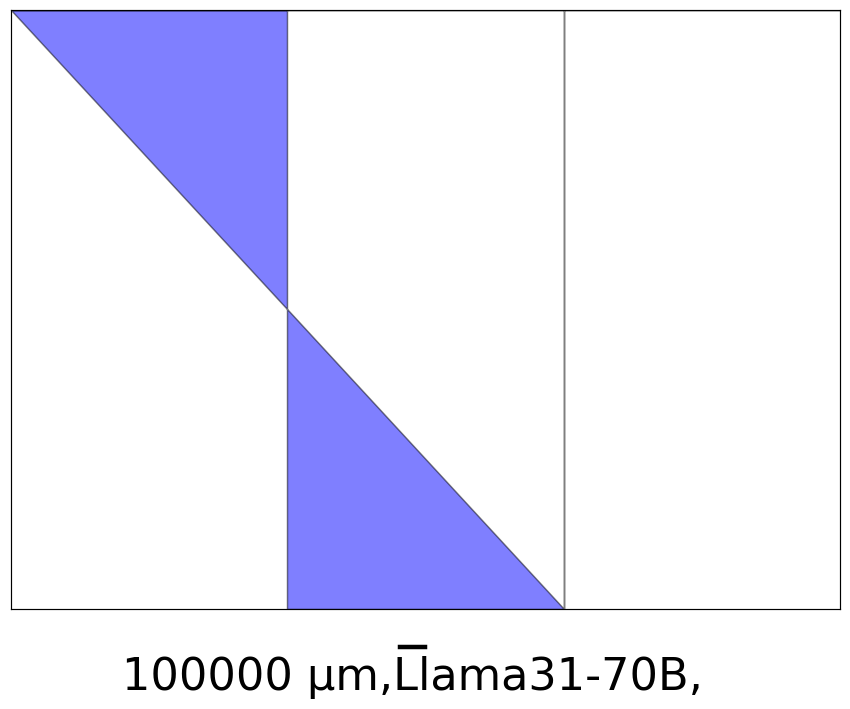
\includegraphics[width=0.13\textwidth]{./pool_all/png/watsonx_meta-llama_llama-3-1-70b-instruct_results/Arrow.png} & 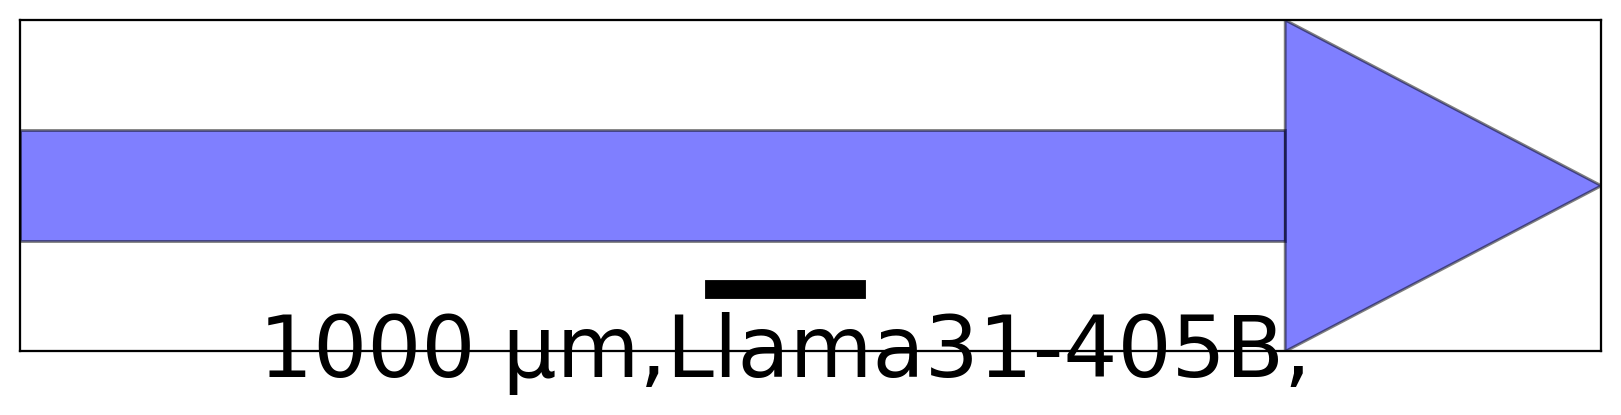
\includegraphics[width=0.13\textwidth]{./pool_all/png/watsonx_meta-llama_llama-3-405b-instruct_results/Arrow.png} \\
      \begin{tabular}{@{}c@{}}Single LLM \\ Baseline \\ Run 1\end{tabular} & 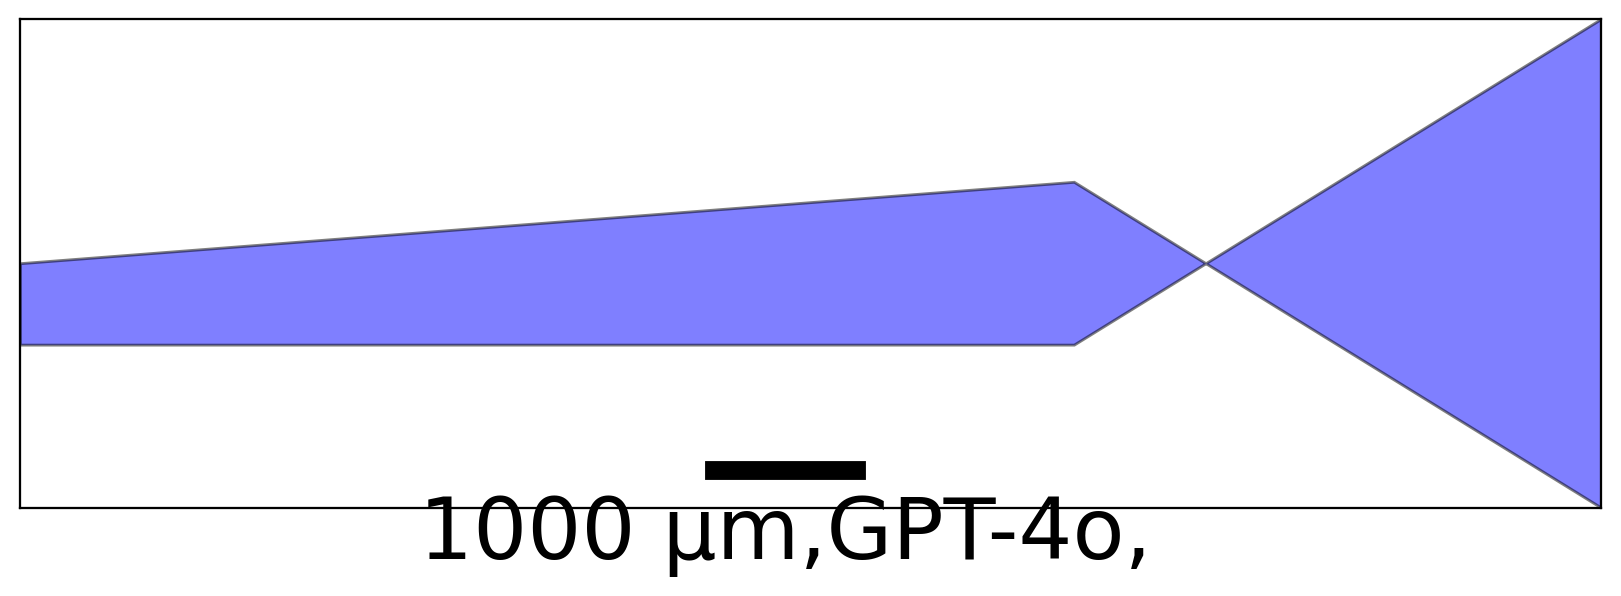
\includegraphics[width=0.13\textwidth]{./run_1/png/gpt-4o_results/Arrow.png} & 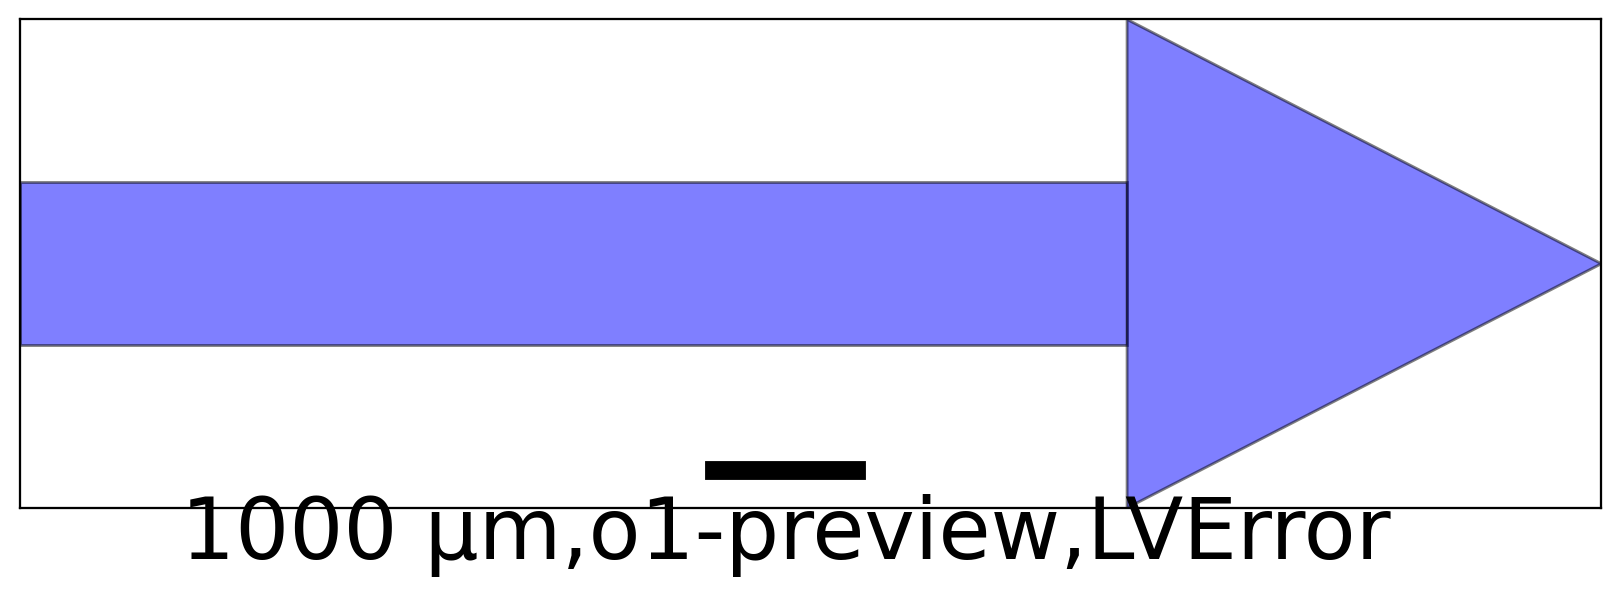
\includegraphics[width=0.13\textwidth]{./run_1/png/o1-preview_results/Arrow.png} & 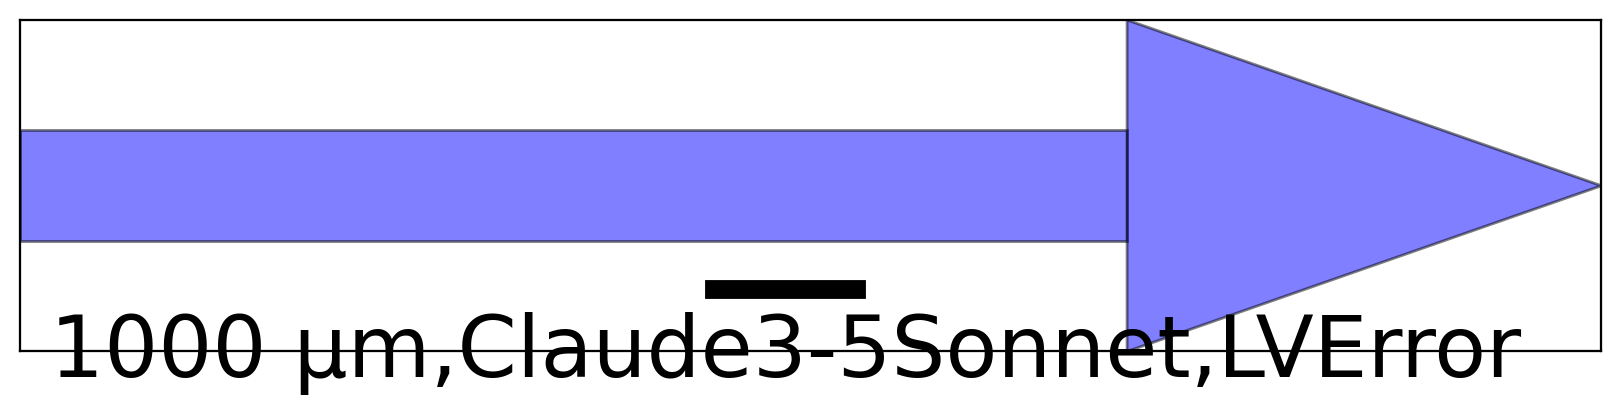
\includegraphics[width=0.13\textwidth]{./run_1/png/claude-3-5-sonnet-20240620_results/Arrow.png} & 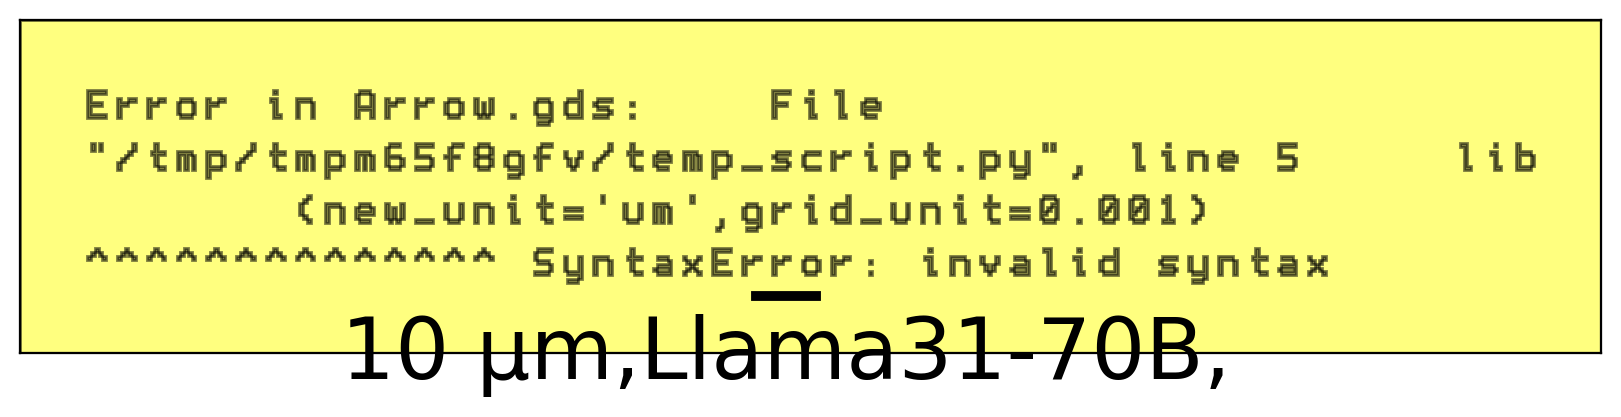
\includegraphics[width=0.13\textwidth]{./run_1/png/watsonx_meta-llama_llama-3-1-70b-instruct_results/Arrow.png} & 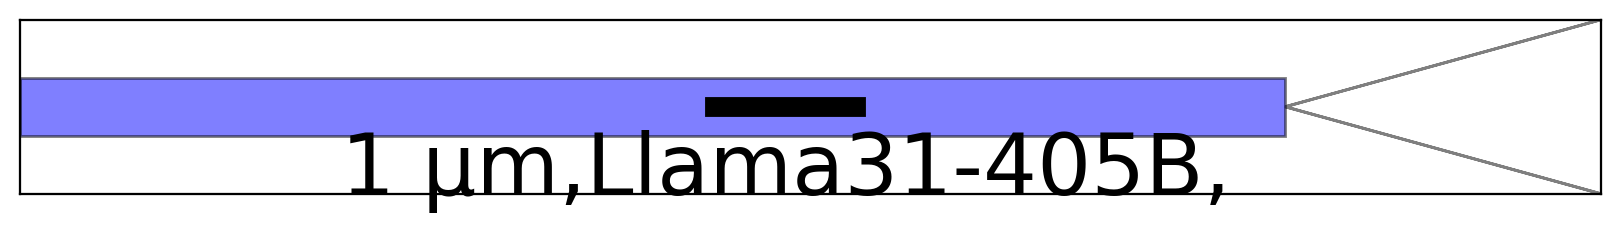
\includegraphics[width=0.13\textwidth]{./run_1/png/watsonx_meta-llama_llama-3-405b-instruct_results/Arrow.png} \\
      \begin{tabular}{@{}c@{}}Single LLM \\ Baseline \\ Run 2\end{tabular} & 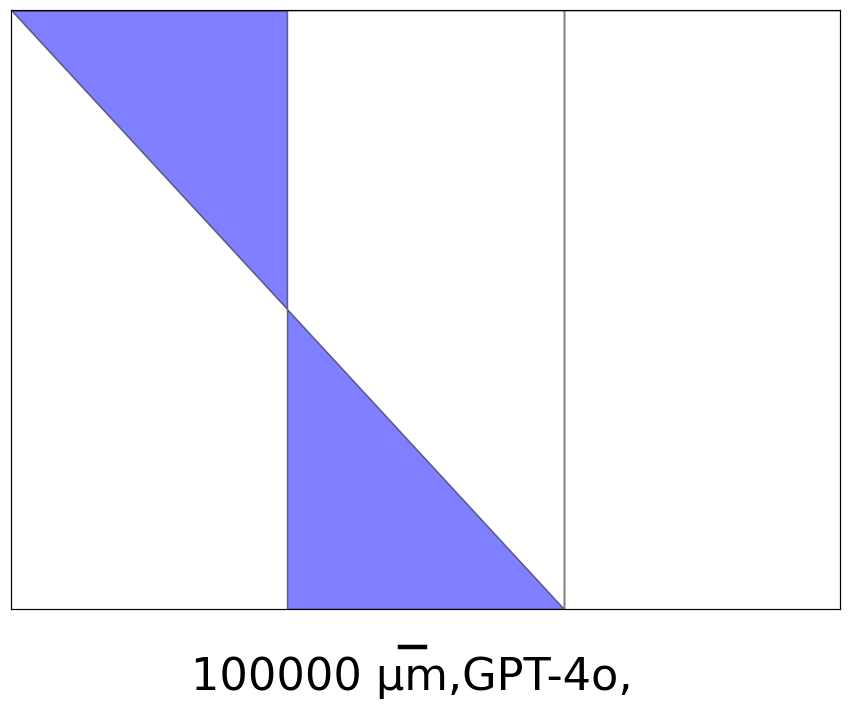
\includegraphics[width=0.13\textwidth]{./run_2/png/gpt-4o_results/Arrow.png} & 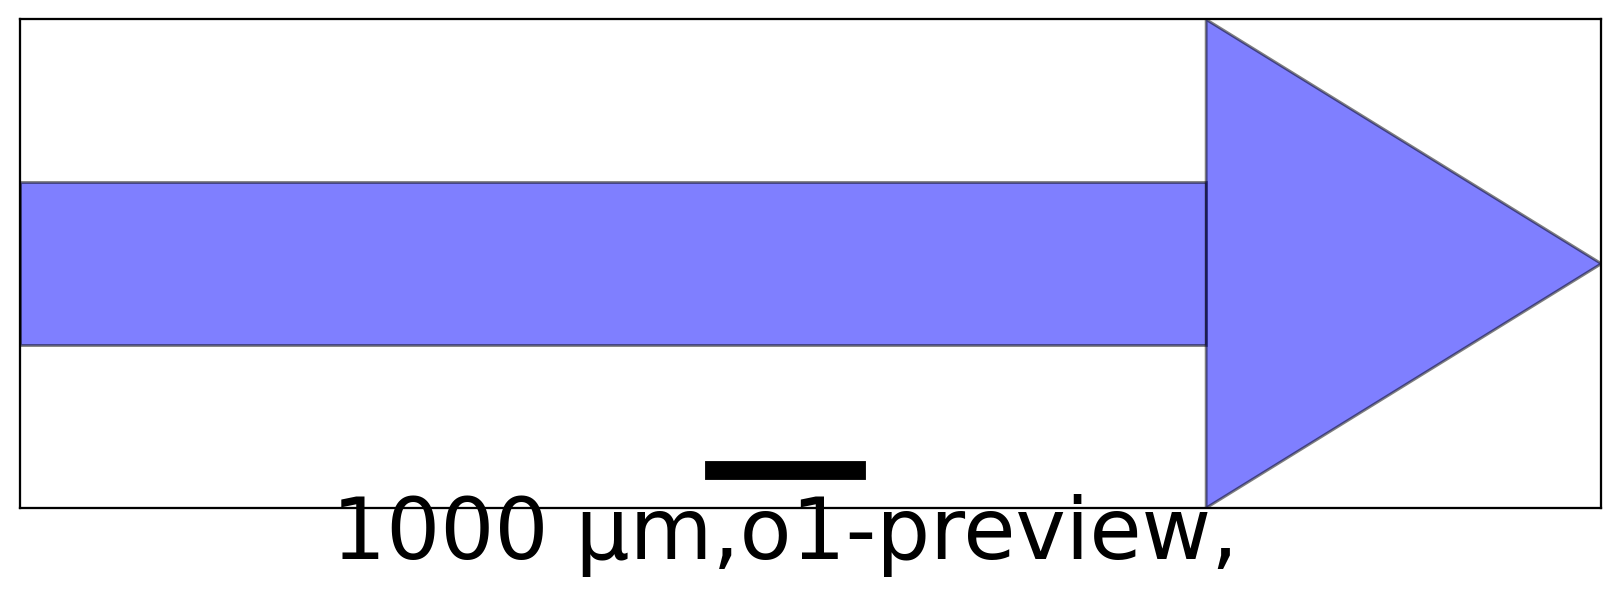
\includegraphics[width=0.13\textwidth]{./run_2/png/o1-preview_results/Arrow.png} & 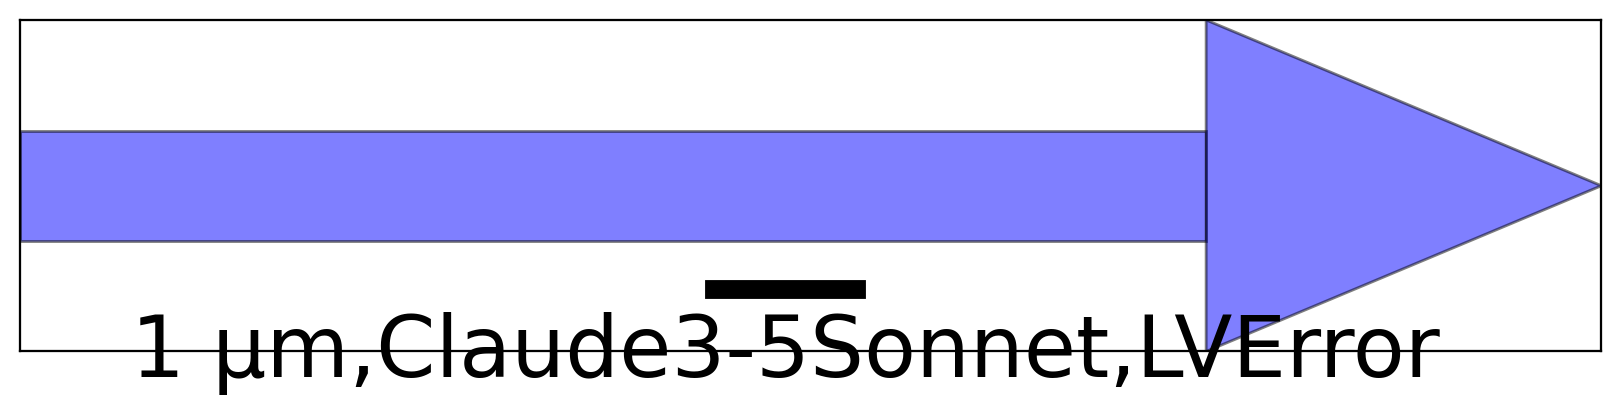
\includegraphics[width=0.13\textwidth]{./run_2/png/claude-3-5-sonnet-20240620_results/Arrow.png} & 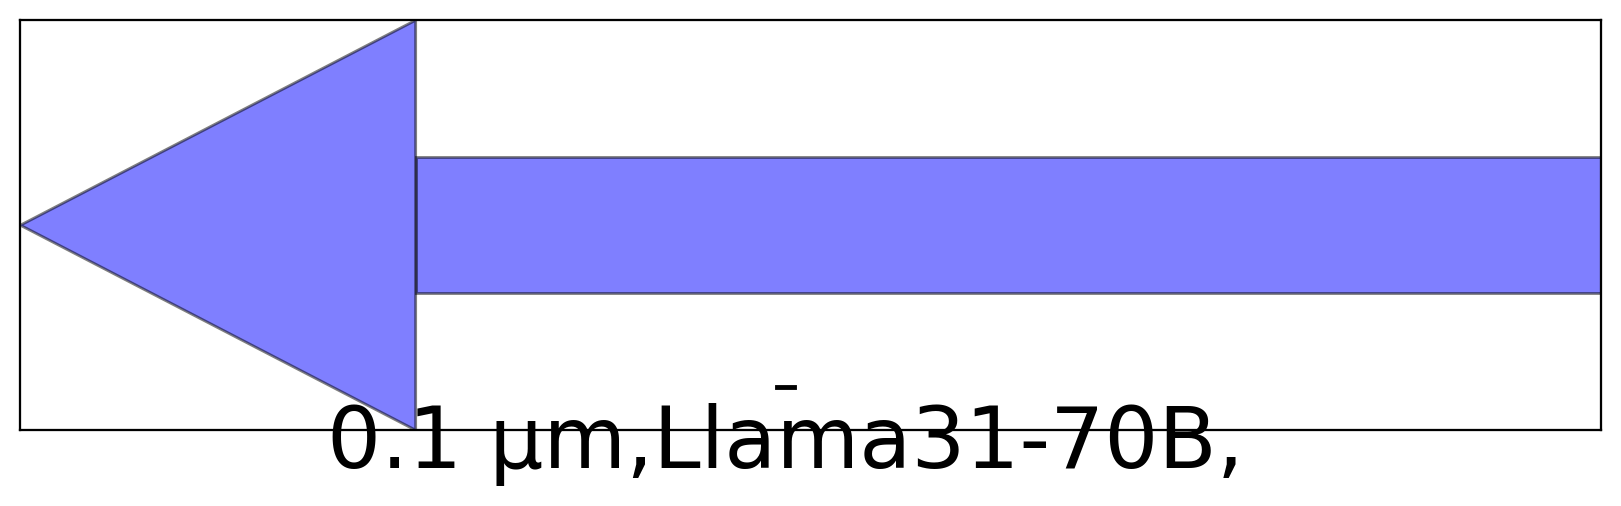
\includegraphics[width=0.13\textwidth]{./run_2/png/watsonx_meta-llama_llama-3-1-70b-instruct_results/Arrow.png} & 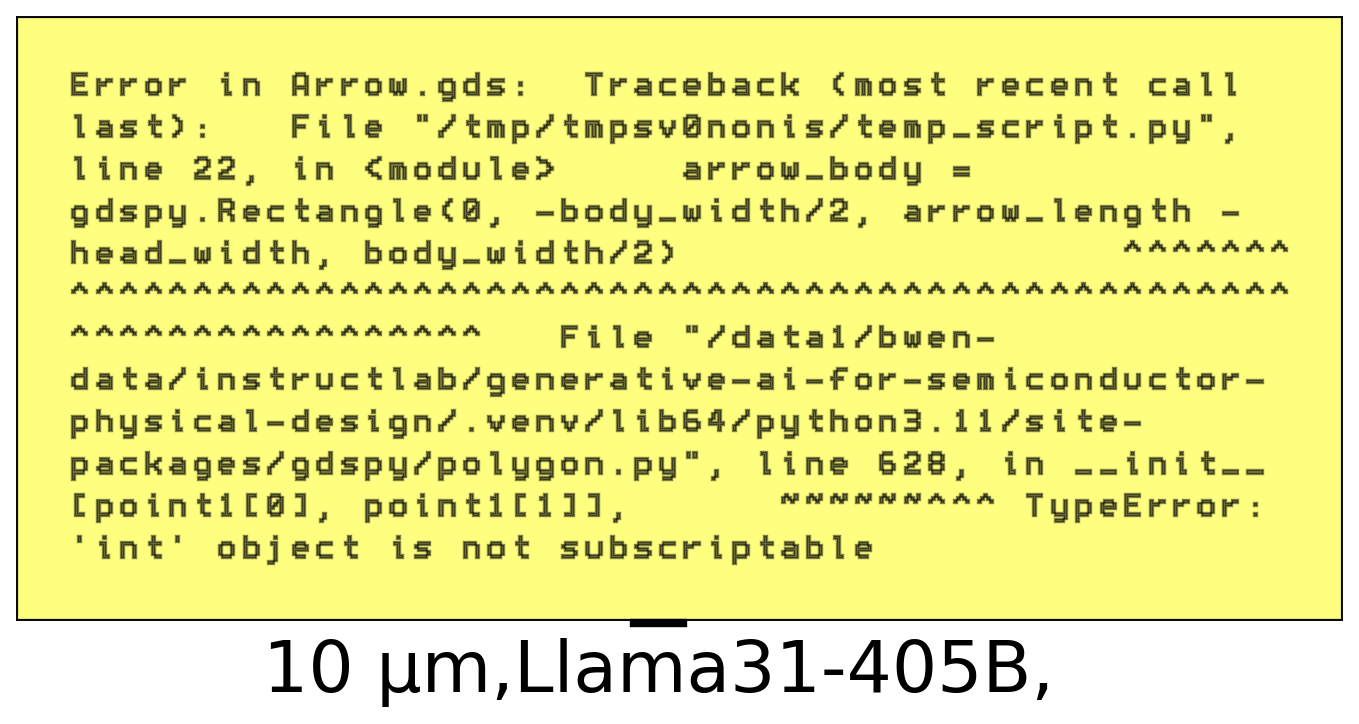
\includegraphics[width=0.13\textwidth]{./run_2/png/watsonx_meta-llama_llama-3-405b-instruct_results/Arrow.png} \\
      \begin{tabular}{@{}c@{}}Single LLM \\ Baseline \\ Run 3\end{tabular} & 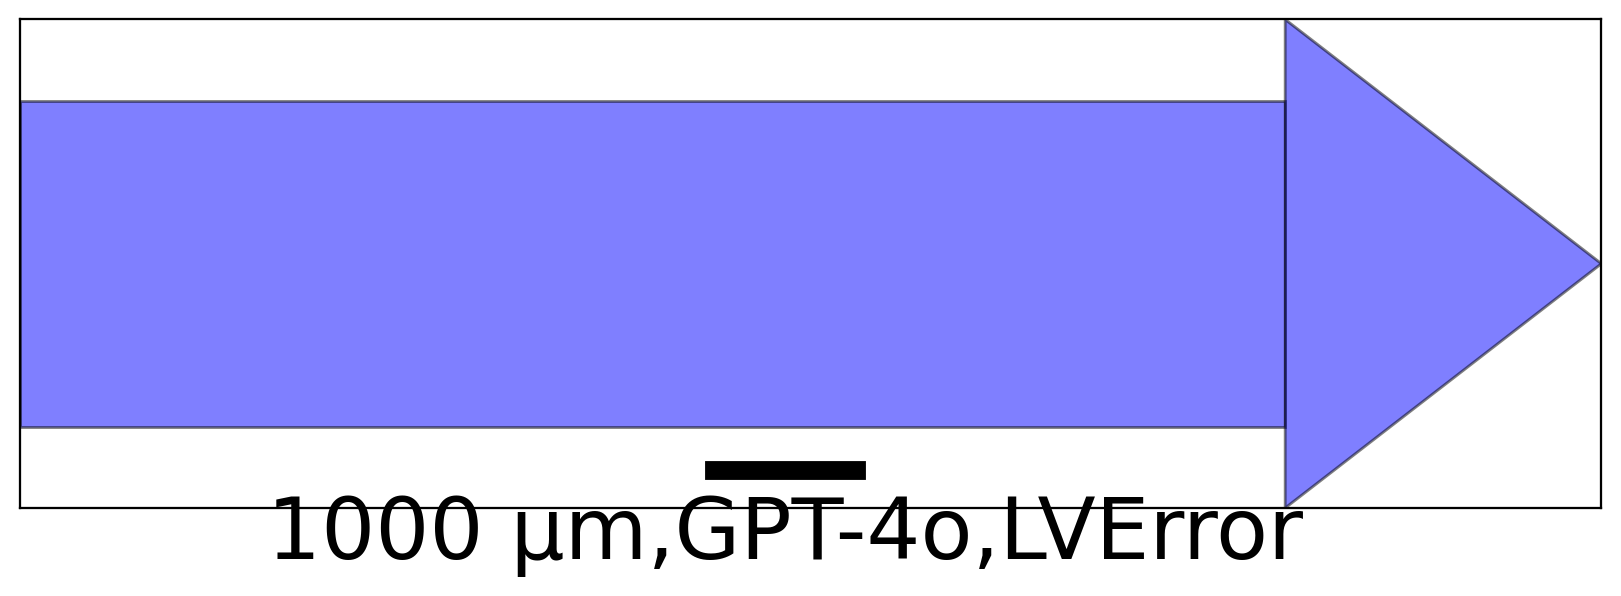
\includegraphics[width=0.13\textwidth]{./run_3/png/gpt-4o_results/Arrow.png} & 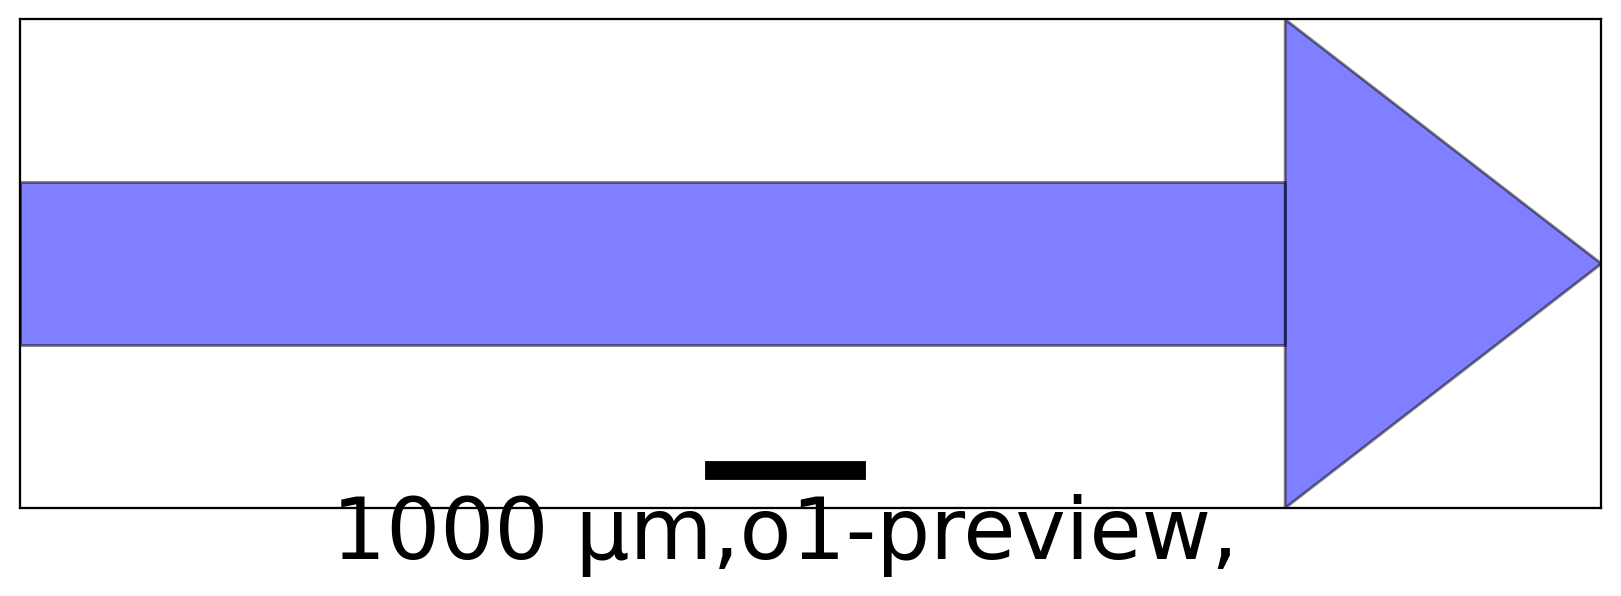
\includegraphics[width=0.13\textwidth]{./run_3/png/o1-preview_results/Arrow.png} & 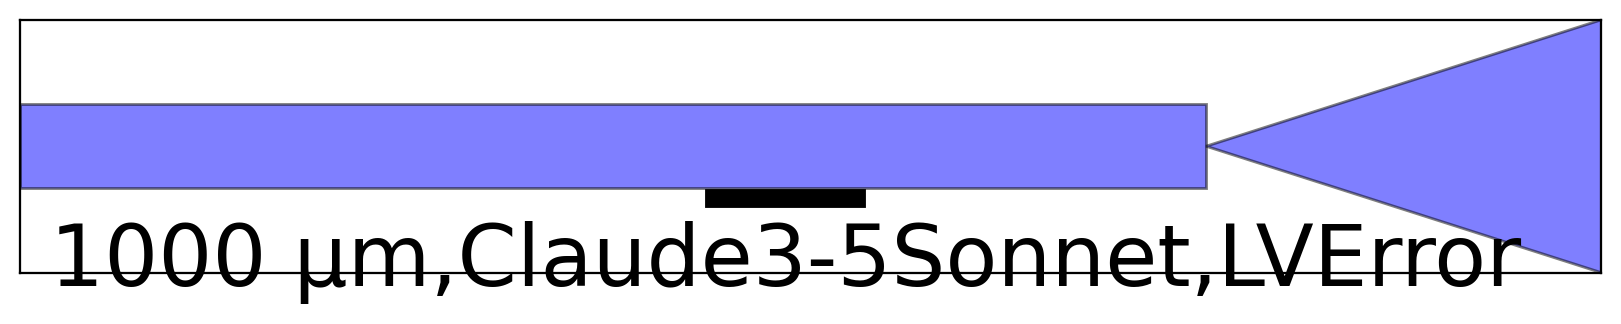
\includegraphics[width=0.13\textwidth]{./run_3/png/claude-3-5-sonnet-20240620_results/Arrow.png} & 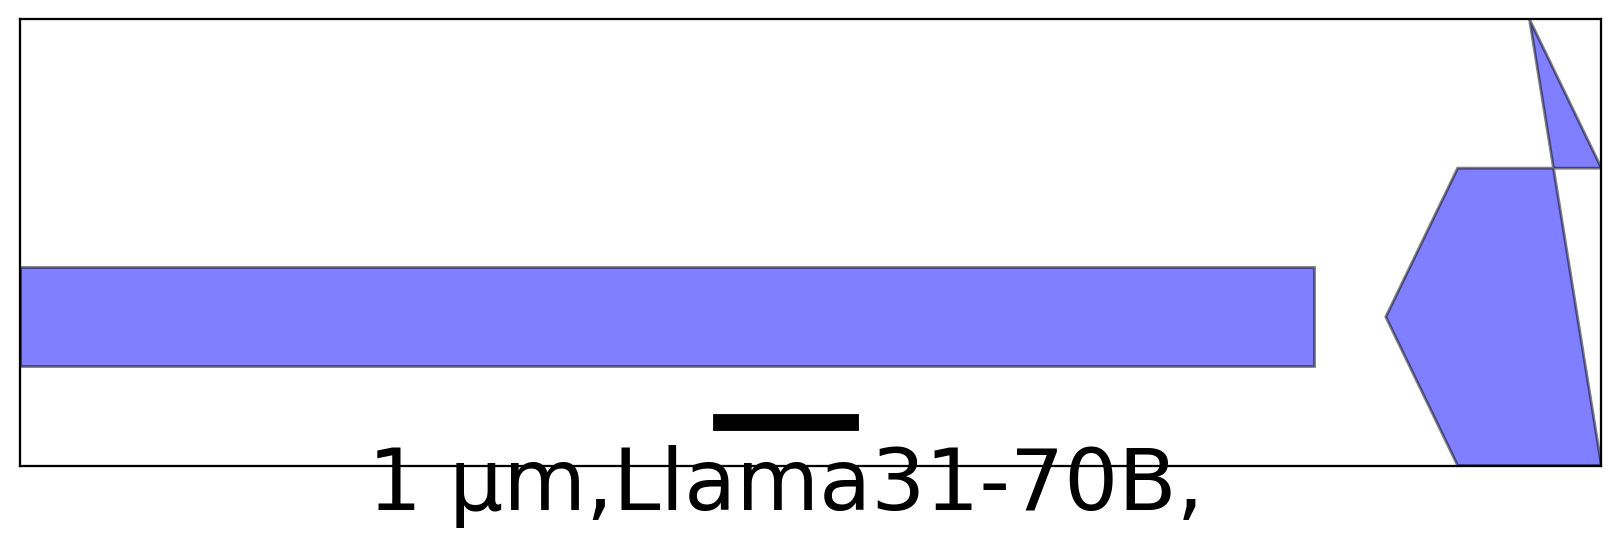
\includegraphics[width=0.13\textwidth]{./run_3/png/watsonx_meta-llama_llama-3-1-70b-instruct_results/Arrow.png} & 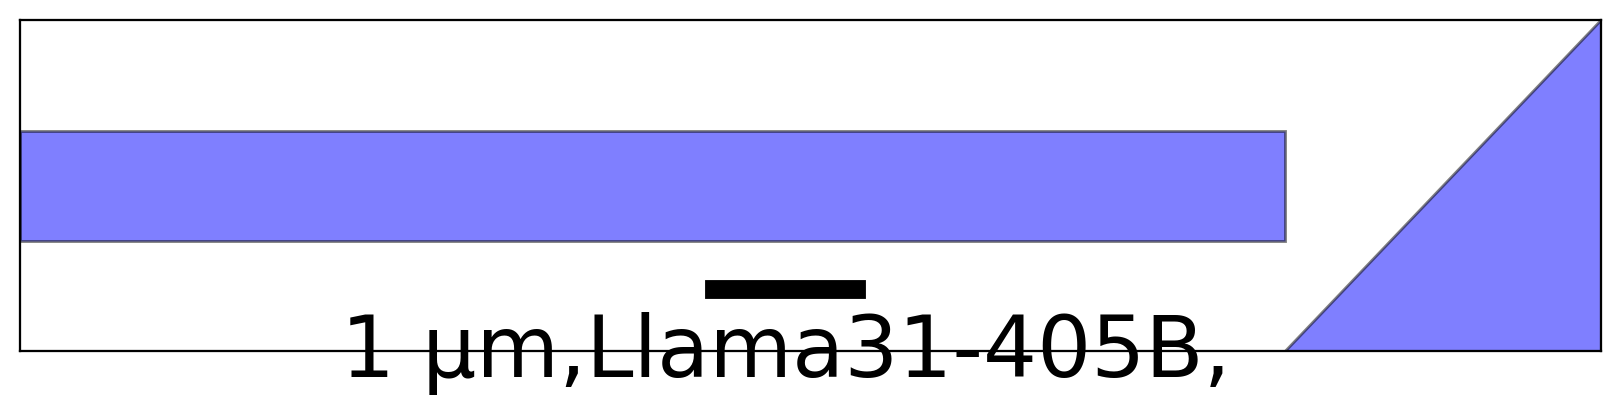
\includegraphics[width=0.13\textwidth]{./run_3/png/watsonx_meta-llama_llama-3-405b-instruct_results/Arrow.png} \\
      \begin{tabular}{@{}c@{}}Single LLM \\ Baseline \\ Run 4\end{tabular} & \includegraphics[width=0.13\textwidth]{./run_4/png/gpt-4o_results/Arrow.png} & \includegraphics[width=0.13\textwidth]{./run_4/png/o1-preview_results/Arrow.png} & \includegraphics[width=0.13\textwidth]{./run_4/png/claude-3-5-sonnet-20240620_results/Arrow.png} & \includegraphics[width=0.13\textwidth]{./run_4/png/watsonx_meta-llama_llama-3-1-70b-instruct_results/Arrow.png} & \includegraphics[width=0.13\textwidth]{./run_4/png/watsonx_meta-llama_llama-3-405b-instruct_results/Arrow.png} \\
      \begin{tabular}{@{}c@{}}Single LLM \\ Baseline \\ Run 5\end{tabular} & \includegraphics[width=0.13\textwidth]{./run_5/png/gpt-4o_results/Arrow.png} & \includegraphics[width=0.13\textwidth]{./run_5/png/o1-preview_results/Arrow.png} & \includegraphics[width=0.13\textwidth]{./run_5/png/claude-3-5-sonnet-20240620_results/Arrow.png} & \includegraphics[width=0.13\textwidth]{./run_5/png/watsonx_meta-llama_llama-3-1-70b-instruct_results/Arrow.png} & \includegraphics[width=0.13\textwidth]{./run_5/png/watsonx_meta-llama_llama-3-405b-instruct_results/Arrow.png} \\
      \bottomrule
    \end{tabularx}
    \caption{Arrow Task Question: Generate an Arrow pointing to the right with length 10 mm, make the body 1/3 width of the head, start at 0,0.}
  \end{table}
  
  \begin{table}
    \label{table:basiclayout}
    \centering
    \begin{tabularx}{0.9\textwidth}{@{}XXXXXX@{}}
      \toprule
      \begin{tabular}{@{}c@{}}Ground Truth \\ \includegraphics[width=0.13\textwidth]{examples_png/BasicLayout.png}\end{tabular} & GPT-4o & Claude-3.5 & Llama-3-70B & Llama-3-405B & o1-preview \\
      \midrule
      SOLOMON & \includegraphics[width=0.13\textwidth]{./pool_all/png/gpt-4o_results/BasicLayout.png} &  & \includegraphics[width=0.13\textwidth]{./pool_all/png/claude-3-5-sonnet-20240620_results/BasicLayout.png} & \includegraphics[width=0.13\textwidth]{./pool_all/png/watsonx_meta-llama_llama-3-1-70b-instruct_results/BasicLayout.png} & \includegraphics[width=0.13\textwidth]{./pool_all/png/watsonx_meta-llama_llama-3-405b-instruct_results/BasicLayout.png} \\
      \begin{tabular}{@{}c@{}}Single LLM \\ Baseline \\ Run 1\end{tabular} & \includegraphics[width=0.13\textwidth]{./run_1/png/gpt-4o_results/BasicLayout.png} & \includegraphics[width=0.13\textwidth]{./run_1/png/o1-preview_results/BasicLayout.png} & \includegraphics[width=0.13\textwidth]{./run_1/png/claude-3-5-sonnet-20240620_results/BasicLayout.png} & \includegraphics[width=0.13\textwidth]{./run_1/png/watsonx_meta-llama_llama-3-1-70b-instruct_results/BasicLayout.png} & \includegraphics[width=0.13\textwidth]{./run_1/png/watsonx_meta-llama_llama-3-405b-instruct_results/BasicLayout.png} \\
      \begin{tabular}{@{}c@{}}Single LLM \\ Baseline \\ Run 2\end{tabular} & \includegraphics[width=0.13\textwidth]{./run_2/png/gpt-4o_results/BasicLayout.png} & \includegraphics[width=0.13\textwidth]{./run_2/png/o1-preview_results/BasicLayout.png} & \includegraphics[width=0.13\textwidth]{./run_2/png/claude-3-5-sonnet-20240620_results/BasicLayout.png} & \includegraphics[width=0.13\textwidth]{./run_2/png/watsonx_meta-llama_llama-3-1-70b-instruct_results/BasicLayout.png} & \includegraphics[width=0.13\textwidth]{./run_2/png/watsonx_meta-llama_llama-3-405b-instruct_results/BasicLayout.png} \\
      \begin{tabular}{@{}c@{}}Single LLM \\ Baseline \\ Run 3\end{tabular} & \includegraphics[width=0.13\textwidth]{./run_3/png/gpt-4o_results/BasicLayout.png} & \includegraphics[width=0.13\textwidth]{./run_3/png/o1-preview_results/BasicLayout.png} & \includegraphics[width=0.13\textwidth]{./run_3/png/claude-3-5-sonnet-20240620_results/BasicLayout.png} & \includegraphics[width=0.13\textwidth]{./run_3/png/watsonx_meta-llama_llama-3-1-70b-instruct_results/BasicLayout.png} & \includegraphics[width=0.13\textwidth]{./run_3/png/watsonx_meta-llama_llama-3-405b-instruct_results/BasicLayout.png} \\
      \begin{tabular}{@{}c@{}}Single LLM \\ Baseline \\ Run 4\end{tabular} & \includegraphics[width=0.13\textwidth]{./run_4/png/gpt-4o_results/BasicLayout.png} & \includegraphics[width=0.13\textwidth]{./run_4/png/o1-preview_results/BasicLayout.png} & \includegraphics[width=0.13\textwidth]{./run_4/png/claude-3-5-sonnet-20240620_results/BasicLayout.png} & \includegraphics[width=0.13\textwidth]{./run_4/png/watsonx_meta-llama_llama-3-1-70b-instruct_results/BasicLayout.png} & \includegraphics[width=0.13\textwidth]{./run_4/png/watsonx_meta-llama_llama-3-405b-instruct_results/BasicLayout.png} \\
      \begin{tabular}{@{}c@{}}Single LLM \\ Baseline \\ Run 5\end{tabular} & \includegraphics[width=0.13\textwidth]{./run_5/png/gpt-4o_results/BasicLayout.png} & \includegraphics[width=0.13\textwidth]{./run_5/png/o1-preview_results/BasicLayout.png} & \includegraphics[width=0.13\textwidth]{./run_5/png/claude-3-5-sonnet-20240620_results/BasicLayout.png} & \includegraphics[width=0.13\textwidth]{./run_5/png/watsonx_meta-llama_llama-3-1-70b-instruct_results/BasicLayout.png} & \includegraphics[width=0.13\textwidth]{./run_5/png/watsonx_meta-llama_llama-3-405b-instruct_results/BasicLayout.png} \\
      \bottomrule
    \end{tabularx}
    \caption{BasicLayout Task Question: 1. Draw a rectangular active region with dimensions 10 µm x 5 µm.
  2. Place a polysilicon gate that crosses the active region vertically at its center, with a width of 1 µm.
  3. Add two square contact holes, each 1 µm x 1 µm, positioned 1 µm away from the gate on either side along the active region.}
  \end{table}
  
  \begin{table}
    \label{table:viaconnection}
    \centering
    \begin{tabularx}{0.9\textwidth}{@{}XXXXXX@{}}
      \toprule
      \begin{tabular}{@{}c@{}}Ground Truth \\ \includegraphics[width=0.13\textwidth]{examples_png/ViaConnection.png}\end{tabular} & GPT-4o & Claude-3.5 & Llama-3-70B & Llama-3-405B & o1-preview \\
      \midrule
      SOLOMON & \includegraphics[width=0.13\textwidth]{./pool_all/png/gpt-4o_results/ViaConnection.png} &  & \includegraphics[width=0.13\textwidth]{./pool_all/png/claude-3-5-sonnet-20240620_results/ViaConnection.png} & \includegraphics[width=0.13\textwidth]{./pool_all/png/watsonx_meta-llama_llama-3-1-70b-instruct_results/ViaConnection.png} & \includegraphics[width=0.13\textwidth]{./pool_all/png/watsonx_meta-llama_llama-3-405b-instruct_results/ViaConnection.png} \\
      \begin{tabular}{@{}c@{}}Single LLM \\ Baseline \\ Run 1\end{tabular} & \includegraphics[width=0.13\textwidth]{./run_1/png/gpt-4o_results/ViaConnection.png} & \includegraphics[width=0.13\textwidth]{./run_1/png/o1-preview_results/ViaConnection.png} & \includegraphics[width=0.13\textwidth]{./run_1/png/claude-3-5-sonnet-20240620_results/ViaConnection.png} & \includegraphics[width=0.13\textwidth]{./run_1/png/watsonx_meta-llama_llama-3-1-70b-instruct_results/ViaConnection.png} & \includegraphics[width=0.13\textwidth]{./run_1/png/watsonx_meta-llama_llama-3-405b-instruct_results/ViaConnection.png} \\
      \begin{tabular}{@{}c@{}}Single LLM \\ Baseline \\ Run 2\end{tabular} & \includegraphics[width=0.13\textwidth]{./run_2/png/gpt-4o_results/ViaConnection.png} & \includegraphics[width=0.13\textwidth]{./run_2/png/o1-preview_results/ViaConnection.png} & \includegraphics[width=0.13\textwidth]{./run_2/png/claude-3-5-sonnet-20240620_results/ViaConnection.png} & \includegraphics[width=0.13\textwidth]{./run_2/png/watsonx_meta-llama_llama-3-1-70b-instruct_results/ViaConnection.png} & \includegraphics[width=0.13\textwidth]{./run_2/png/watsonx_meta-llama_llama-3-405b-instruct_results/ViaConnection.png} \\
      \begin{tabular}{@{}c@{}}Single LLM \\ Baseline \\ Run 3\end{tabular} & \includegraphics[width=0.13\textwidth]{./run_3/png/gpt-4o_results/ViaConnection.png} & \includegraphics[width=0.13\textwidth]{./run_3/png/o1-preview_results/ViaConnection.png} & \includegraphics[width=0.13\textwidth]{./run_3/png/claude-3-5-sonnet-20240620_results/ViaConnection.png} & \includegraphics[width=0.13\textwidth]{./run_3/png/watsonx_meta-llama_llama-3-1-70b-instruct_results/ViaConnection.png} & \includegraphics[width=0.13\textwidth]{./run_3/png/watsonx_meta-llama_llama-3-405b-instruct_results/ViaConnection.png} \\
      \begin{tabular}{@{}c@{}}Single LLM \\ Baseline \\ Run 4\end{tabular} & \includegraphics[width=0.13\textwidth]{./run_4/png/gpt-4o_results/ViaConnection.png} & \includegraphics[width=0.13\textwidth]{./run_4/png/o1-preview_results/ViaConnection.png} & \includegraphics[width=0.13\textwidth]{./run_4/png/claude-3-5-sonnet-20240620_results/ViaConnection.png} & \includegraphics[width=0.13\textwidth]{./run_4/png/watsonx_meta-llama_llama-3-1-70b-instruct_results/ViaConnection.png} & \includegraphics[width=0.13\textwidth]{./run_4/png/watsonx_meta-llama_llama-3-405b-instruct_results/ViaConnection.png} \\
      \begin{tabular}{@{}c@{}}Single LLM \\ Baseline \\ Run 5\end{tabular} & \includegraphics[width=0.13\textwidth]{./run_5/png/gpt-4o_results/ViaConnection.png} & \includegraphics[width=0.13\textwidth]{./run_5/png/o1-preview_results/ViaConnection.png} & \includegraphics[width=0.13\textwidth]{./run_5/png/claude-3-5-sonnet-20240620_results/ViaConnection.png} & \includegraphics[width=0.13\textwidth]{./run_5/png/watsonx_meta-llama_llama-3-1-70b-instruct_results/ViaConnection.png} & \includegraphics[width=0.13\textwidth]{./run_5/png/watsonx_meta-llama_llama-3-405b-instruct_results/ViaConnection.png} \\
      \bottomrule
    \end{tabularx}
    \caption{ViaConnection Task Question: Create a design with three layers: via layer (yellow), metal layer (blue), and pad layer (red). The via radius is 10 units, pad radius is 30 units, and metal connection width is 40 units with a total length of 600 units. Position the first via at (50, 150) and the second via at (550, 150). Ensure the metal connection fully covers the vias and leaves a margin of 10 units between the edge of the metal and the pads. Leave a space of 50 units between the vias and the edges of the metal connection.}
  \end{table}
  
  \begin{table}
    \label{table:dldchip}
    \centering
    \begin{tabularx}{0.9\textwidth}{@{}XXXXXX@{}}
      \toprule
      \begin{tabular}{@{}c@{}}Ground Truth \\ \includegraphics[width=0.13\textwidth]{examples_png/DLDChip.png}\end{tabular} & GPT-4o & Claude-3.5 & Llama-3-70B & Llama-3-405B & o1-preview \\
      \midrule
      SOLOMON & \includegraphics[width=0.13\textwidth]{./pool_all/png/gpt-4o_results/DLDChip.png} &  & \includegraphics[width=0.13\textwidth]{./pool_all/png/claude-3-5-sonnet-20240620_results/DLDChip.png} & \includegraphics[width=0.13\textwidth]{./pool_all/png/watsonx_meta-llama_llama-3-1-70b-instruct_results/DLDChip.png} & \includegraphics[width=0.13\textwidth]{./pool_all/png/watsonx_meta-llama_llama-3-405b-instruct_results/DLDChip.png} \\
      \begin{tabular}{@{}c@{}}Single LLM \\ Baseline \\ Run 1\end{tabular} & \includegraphics[width=0.13\textwidth]{./run_1/png/gpt-4o_results/DLDChip.png} & \includegraphics[width=0.13\textwidth]{./run_1/png/o1-preview_results/DLDChip.png} & \includegraphics[width=0.13\textwidth]{./run_1/png/claude-3-5-sonnet-20240620_results/DLDChip.png} & \includegraphics[width=0.13\textwidth]{./run_1/png/watsonx_meta-llama_llama-3-1-70b-instruct_results/DLDChip.png} & \includegraphics[width=0.13\textwidth]{./run_1/png/watsonx_meta-llama_llama-3-405b-instruct_results/DLDChip.png} \\
      \begin{tabular}{@{}c@{}}Single LLM \\ Baseline \\ Run 2\end{tabular} & \includegraphics[width=0.13\textwidth]{./run_2/png/gpt-4o_results/DLDChip.png} & \includegraphics[width=0.13\textwidth]{./run_2/png/o1-preview_results/DLDChip.png} & \includegraphics[width=0.13\textwidth]{./run_2/png/claude-3-5-sonnet-20240620_results/DLDChip.png} & \includegraphics[width=0.13\textwidth]{./run_2/png/watsonx_meta-llama_llama-3-1-70b-instruct_results/DLDChip.png} & \includegraphics[width=0.13\textwidth]{./run_2/png/watsonx_meta-llama_llama-3-405b-instruct_results/DLDChip.png} \\
      \begin{tabular}{@{}c@{}}Single LLM \\ Baseline \\ Run 3\end{tabular} & \includegraphics[width=0.13\textwidth]{./run_3/png/gpt-4o_results/DLDChip.png} & \includegraphics[width=0.13\textwidth]{./run_3/png/o1-preview_results/DLDChip.png} & \includegraphics[width=0.13\textwidth]{./run_3/png/claude-3-5-sonnet-20240620_results/DLDChip.png} & \includegraphics[width=0.13\textwidth]{./run_3/png/watsonx_meta-llama_llama-3-1-70b-instruct_results/DLDChip.png} & \includegraphics[width=0.13\textwidth]{./run_3/png/watsonx_meta-llama_llama-3-405b-instruct_results/DLDChip.png} \\
      \begin{tabular}{@{}c@{}}Single LLM \\ Baseline \\ Run 4\end{tabular} & \includegraphics[width=0.13\textwidth]{./run_4/png/gpt-4o_results/DLDChip.png} & \includegraphics[width=0.13\textwidth]{./run_4/png/o1-preview_results/DLDChip.png} & \includegraphics[width=0.13\textwidth]{./run_4/png/claude-3-5-sonnet-20240620_results/DLDChip.png} & \includegraphics[width=0.13\textwidth]{./run_4/png/watsonx_meta-llama_llama-3-1-70b-instruct_results/DLDChip.png} & \includegraphics[width=0.13\textwidth]{./run_4/png/watsonx_meta-llama_llama-3-405b-instruct_results/DLDChip.png} \\
      \begin{tabular}{@{}c@{}}Single LLM \\ Baseline \\ Run 5\end{tabular} & \includegraphics[width=0.13\textwidth]{./run_5/png/gpt-4o_results/DLDChip.png} & \includegraphics[width=0.13\textwidth]{./run_5/png/o1-preview_results/DLDChip.png} & \includegraphics[width=0.13\textwidth]{./run_5/png/claude-3-5-sonnet-20240620_results/DLDChip.png} & \includegraphics[width=0.13\textwidth]{./run_5/png/watsonx_meta-llama_llama-3-1-70b-instruct_results/DLDChip.png} & \includegraphics[width=0.13\textwidth]{./run_5/png/watsonx_meta-llama_llama-3-405b-instruct_results/DLDChip.png} \\
      \bottomrule
    \end{tabularx}
    \caption{DLDChip Task Question: Draw a deterministic lateral displacement chip - include channel that can hold the array has gap size = 225 nm, circular pillar size = 400 nm, width = 30 pillars, row shift fraction = 0.1, add an inlet and outlet 40 µm diameter before and after the channel, use a 20*50 µm bus to connect the inlet and outlet to the channel.}
  \end{table}